%#!platex
\documentclass[platex,dvipdfmx]{rbproceedings}
% English option
%\documentclass[platex,dvipdfmx,english]{rbproceedings}
%#!uplatex
%\documentclass[uplatex,dvipdfmx]{rbproceedings}
%#!lualatex
%\documentclass[lualatex]{rbproceedings}

% パッケージ
\usepackage{graphicx,xcolor}  % グラフィックス関連
\usepackage{here}
\usepackage{url}
\usepackage{hyperref}
\hypersetup{
    colorlinks=true,
    citecolor=blue,
    linkcolor=blue,
    urlcolor=blue,
    pdfborder={0 0 0},
}
%\usepackage{jlreq-deluxe}  % 多書体化(otf パッケージは使用しない)、Ubuntu 22.04 以降
\usepackage[verb]{bxghost}  % \verb 前後に適切な和欧文間スペース
\usepackage{pxrubrica}  % ルビ

% 参考文献のフォントサイズを指定
%\renewcommand{\bibfont}{\normalsize}  % 標準サイズ
%\renewcommand{\bibfont}{\footnotesize}  % より小さく

% \emph をゴシックかつ太字に(比較的新しい LaTeX が必要)
\DeclareEmphSequence{\gtfamily\sffamily\bfseries}

% 著者用マクロ
\newcommand{\pkg}[1]{\textsf{#1}}
\newcommand{\code}[1]{\texttt{#1}}
\newcommand{\comment}[1]{\textcolor{red}{#1}}

% タイトル
\title{\pkg{RBProceedings}文書クラス サンプル文書}

\author{%
中村 勇太${}^{1}$,吉田 侑樹${}^{1}$,青木 修平${}^{1}$,村上 オト${}^{1}$\\
${}^{1}$Abudori Lab.
}

%\begin{abstract}
%概要の例文.概要の例文.概要の例文.概要の例文.概要の例文.概要の例文.概要の例文.概要の例文.概要の例文.概要の例文.概要の例文.概要の例文.概要の例文.概要の例文.概要の例文.概要の例文.概要の例文.概要の例文.概要の例文.概要の例文.
%\end{abstract}

% 本文
\begin{document}
\maketitle

\section{はじめに}
つくばチャレンジは2024年のロボット大賞に選出された。
つくばチャレンジは18年間、課題や取り組みを変えながら日本のロボット技術の進歩に大きく貢献してきた。
さまざまな研究者に大体的に実験できる環境を提供しつづけロボットの技術を成長させてきた。
完走しているチームの技術力は非常に高い。
初めて参加するチームや個人で参加するチームとは技術的な差が大きい。
初参加から完走するまでの道のりは遠い。
その要因は以下の点であると感じた。
完走しているチームの多くは高価な3DLiDARを搭載している。
ROS 2を使用した3Dナビゲーションのノウハウがウェブ上にあまり公開されていない。
つくばチャレンジレポートは昨年のレポートの差分が書かれていることが多い。
つくばチャレンジレポートは特定の課題の解法が書かれていることが多い。
つくばチャレンジレポートは過去のレポートがオープンになっていないため、引用先が見られない。
以上の点から、初学者や新規参入者に対して敷居が高いように感じた。
同時に、完走するために必要なことは以下のように感じた。
屋外の自律走行には初学者ほど3DLiDARがあった方がよい。
複雑なシステムを運用するには、質の良いハードウェアが必要である。
OSSを駆使すればある程度まではロボットを動作させることができる。
OSSを利用するだけでは完走には至らない。
AbudoriLab.チームでは、本走行では確認走行区間をクリアできなかった。
他のロボットが通路を塞いだため新ルートを作れなかった。
決められたルートに何も障害物がない状態であれば、もっと走行することができた。
決められたルートを走行することだけであれば、自己位置を喪失することなく、障害物も発見し走行することができた。
ゼロからつくばチャレンジに参加する人に必要なことがわかるレポートにしたい。
AbudoriLab.が用意したロボットやソフトウェア構成を紹介する。
\begin{figure*}[htbp]
    \centering
    \begin{minipage}[b]{0.45\hsize}
       \centering
       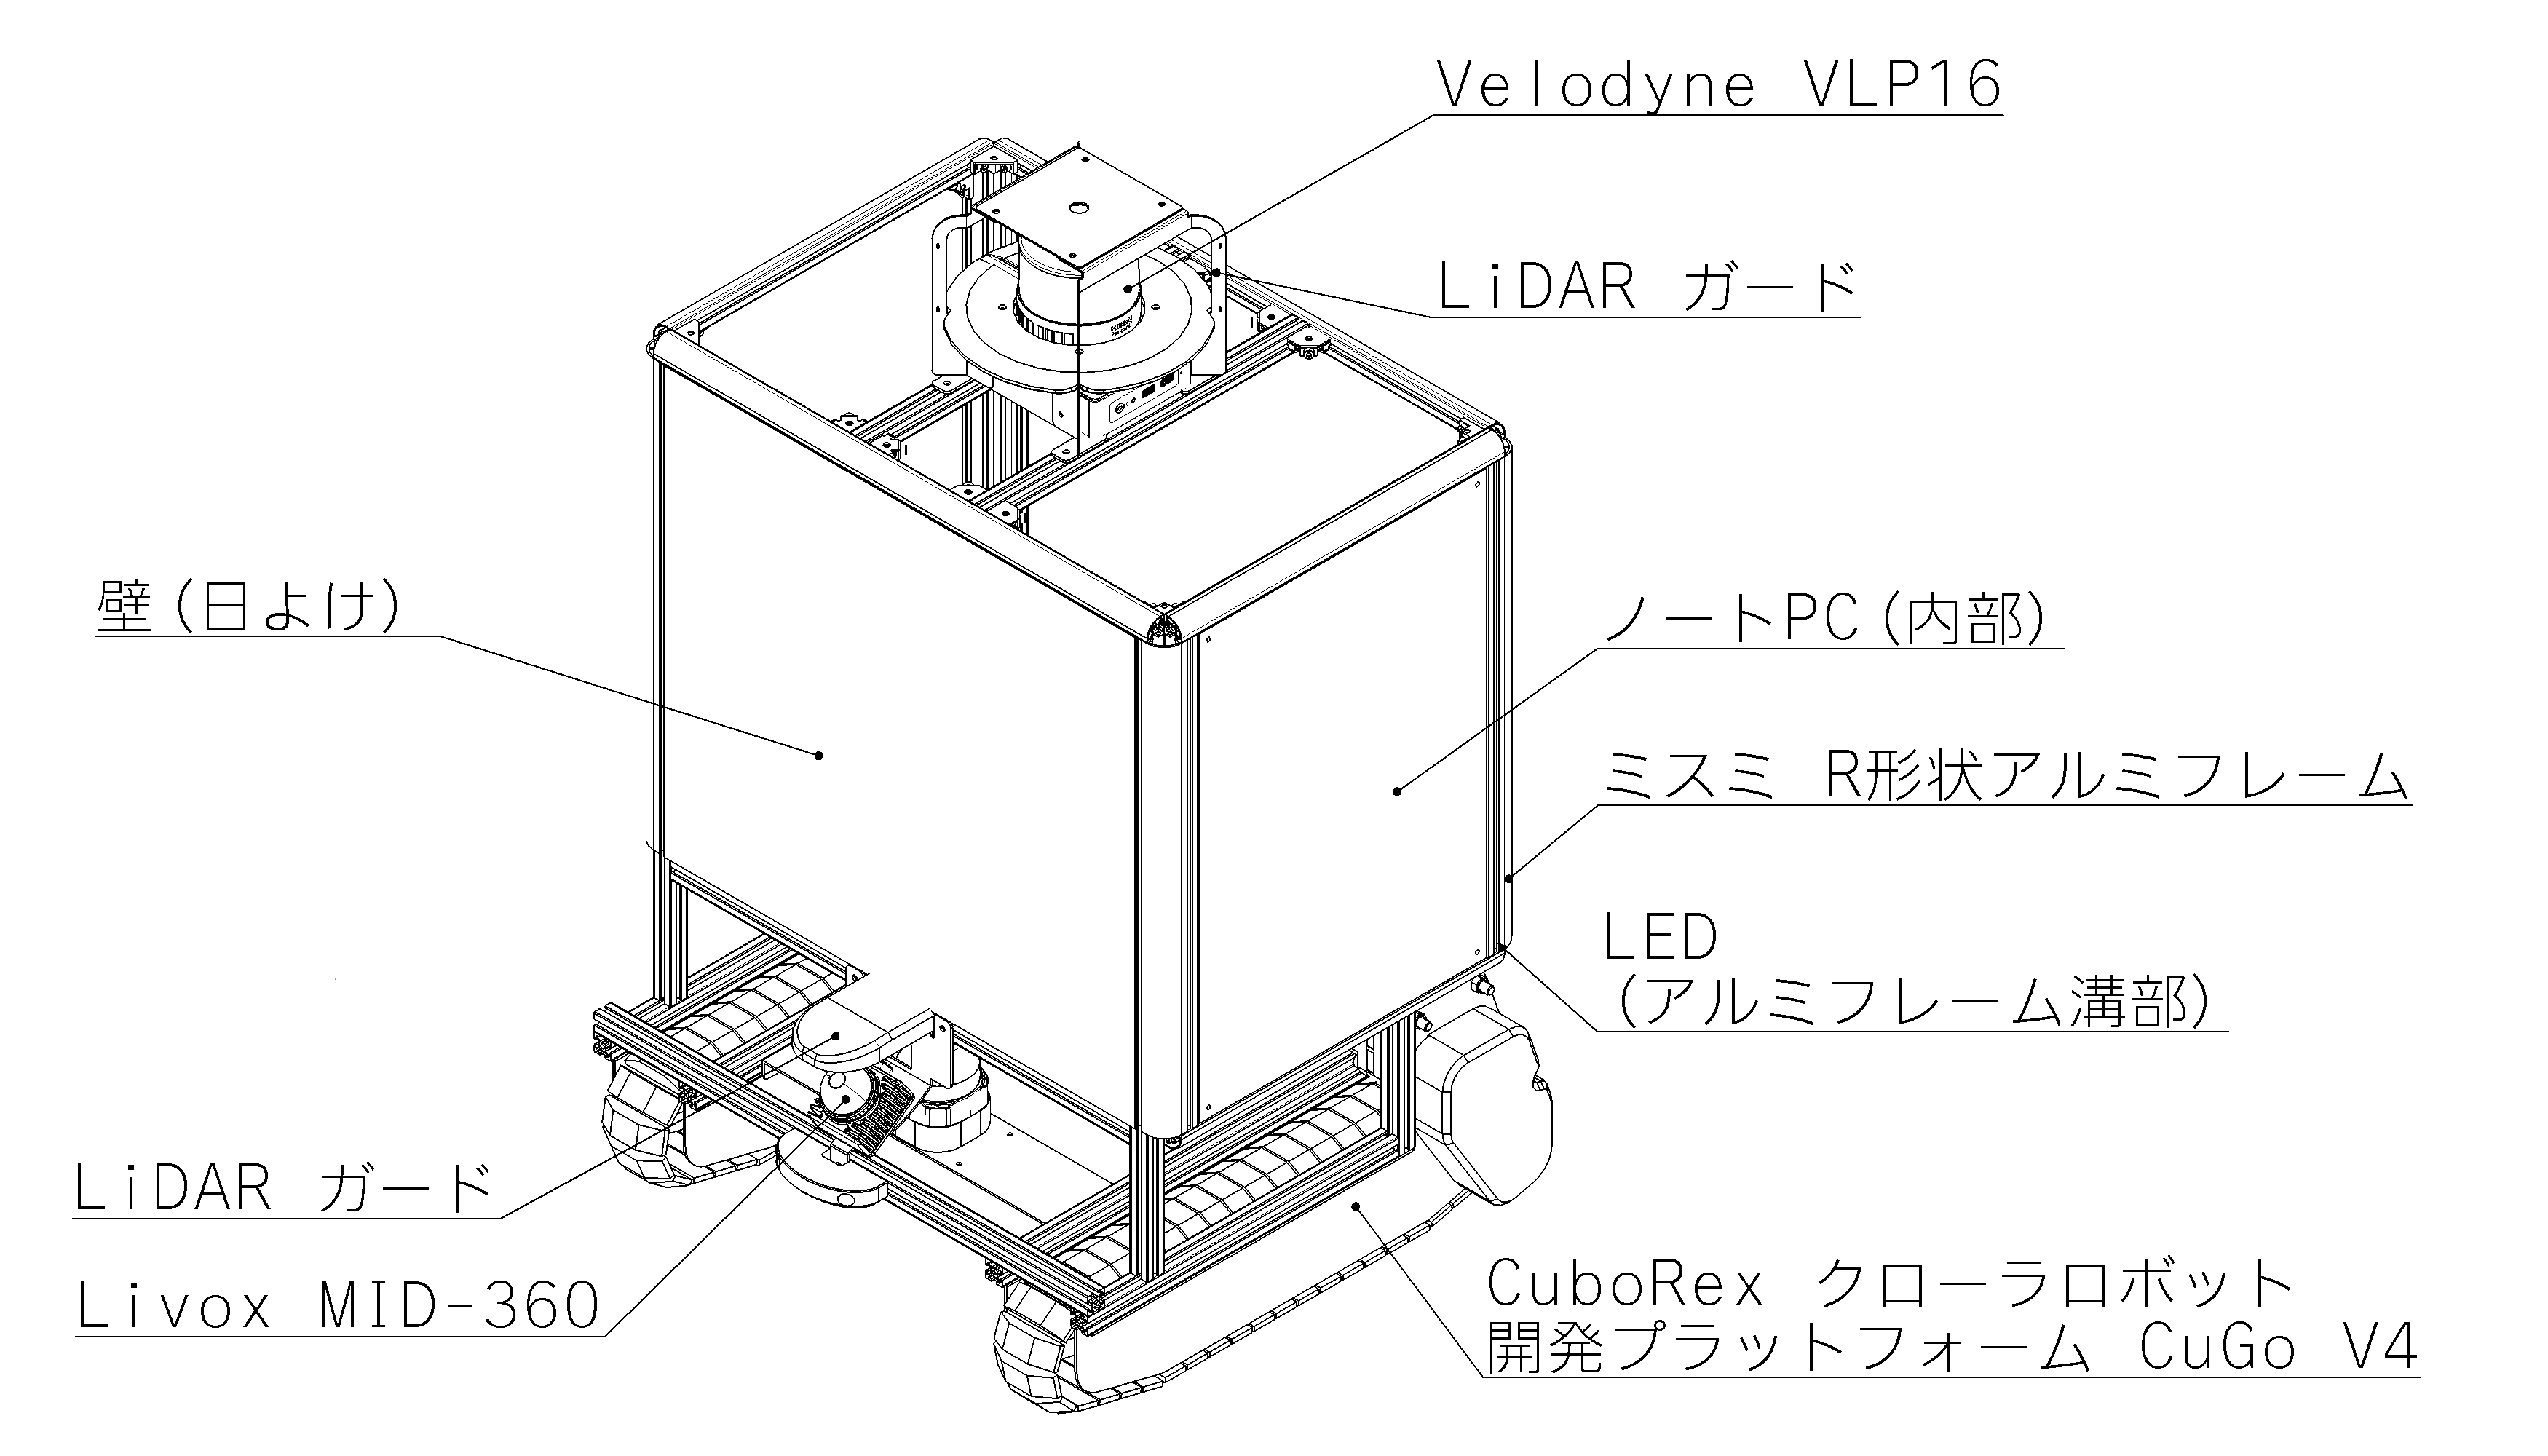
\includegraphics[width=\hsize]{fig/component_parts.png}
       \caption{左の図}
       \label{fig:hidari}
    \end{minipage}
  %
    \begin{minipage}[b]{0.25\hsize}
       \centering
       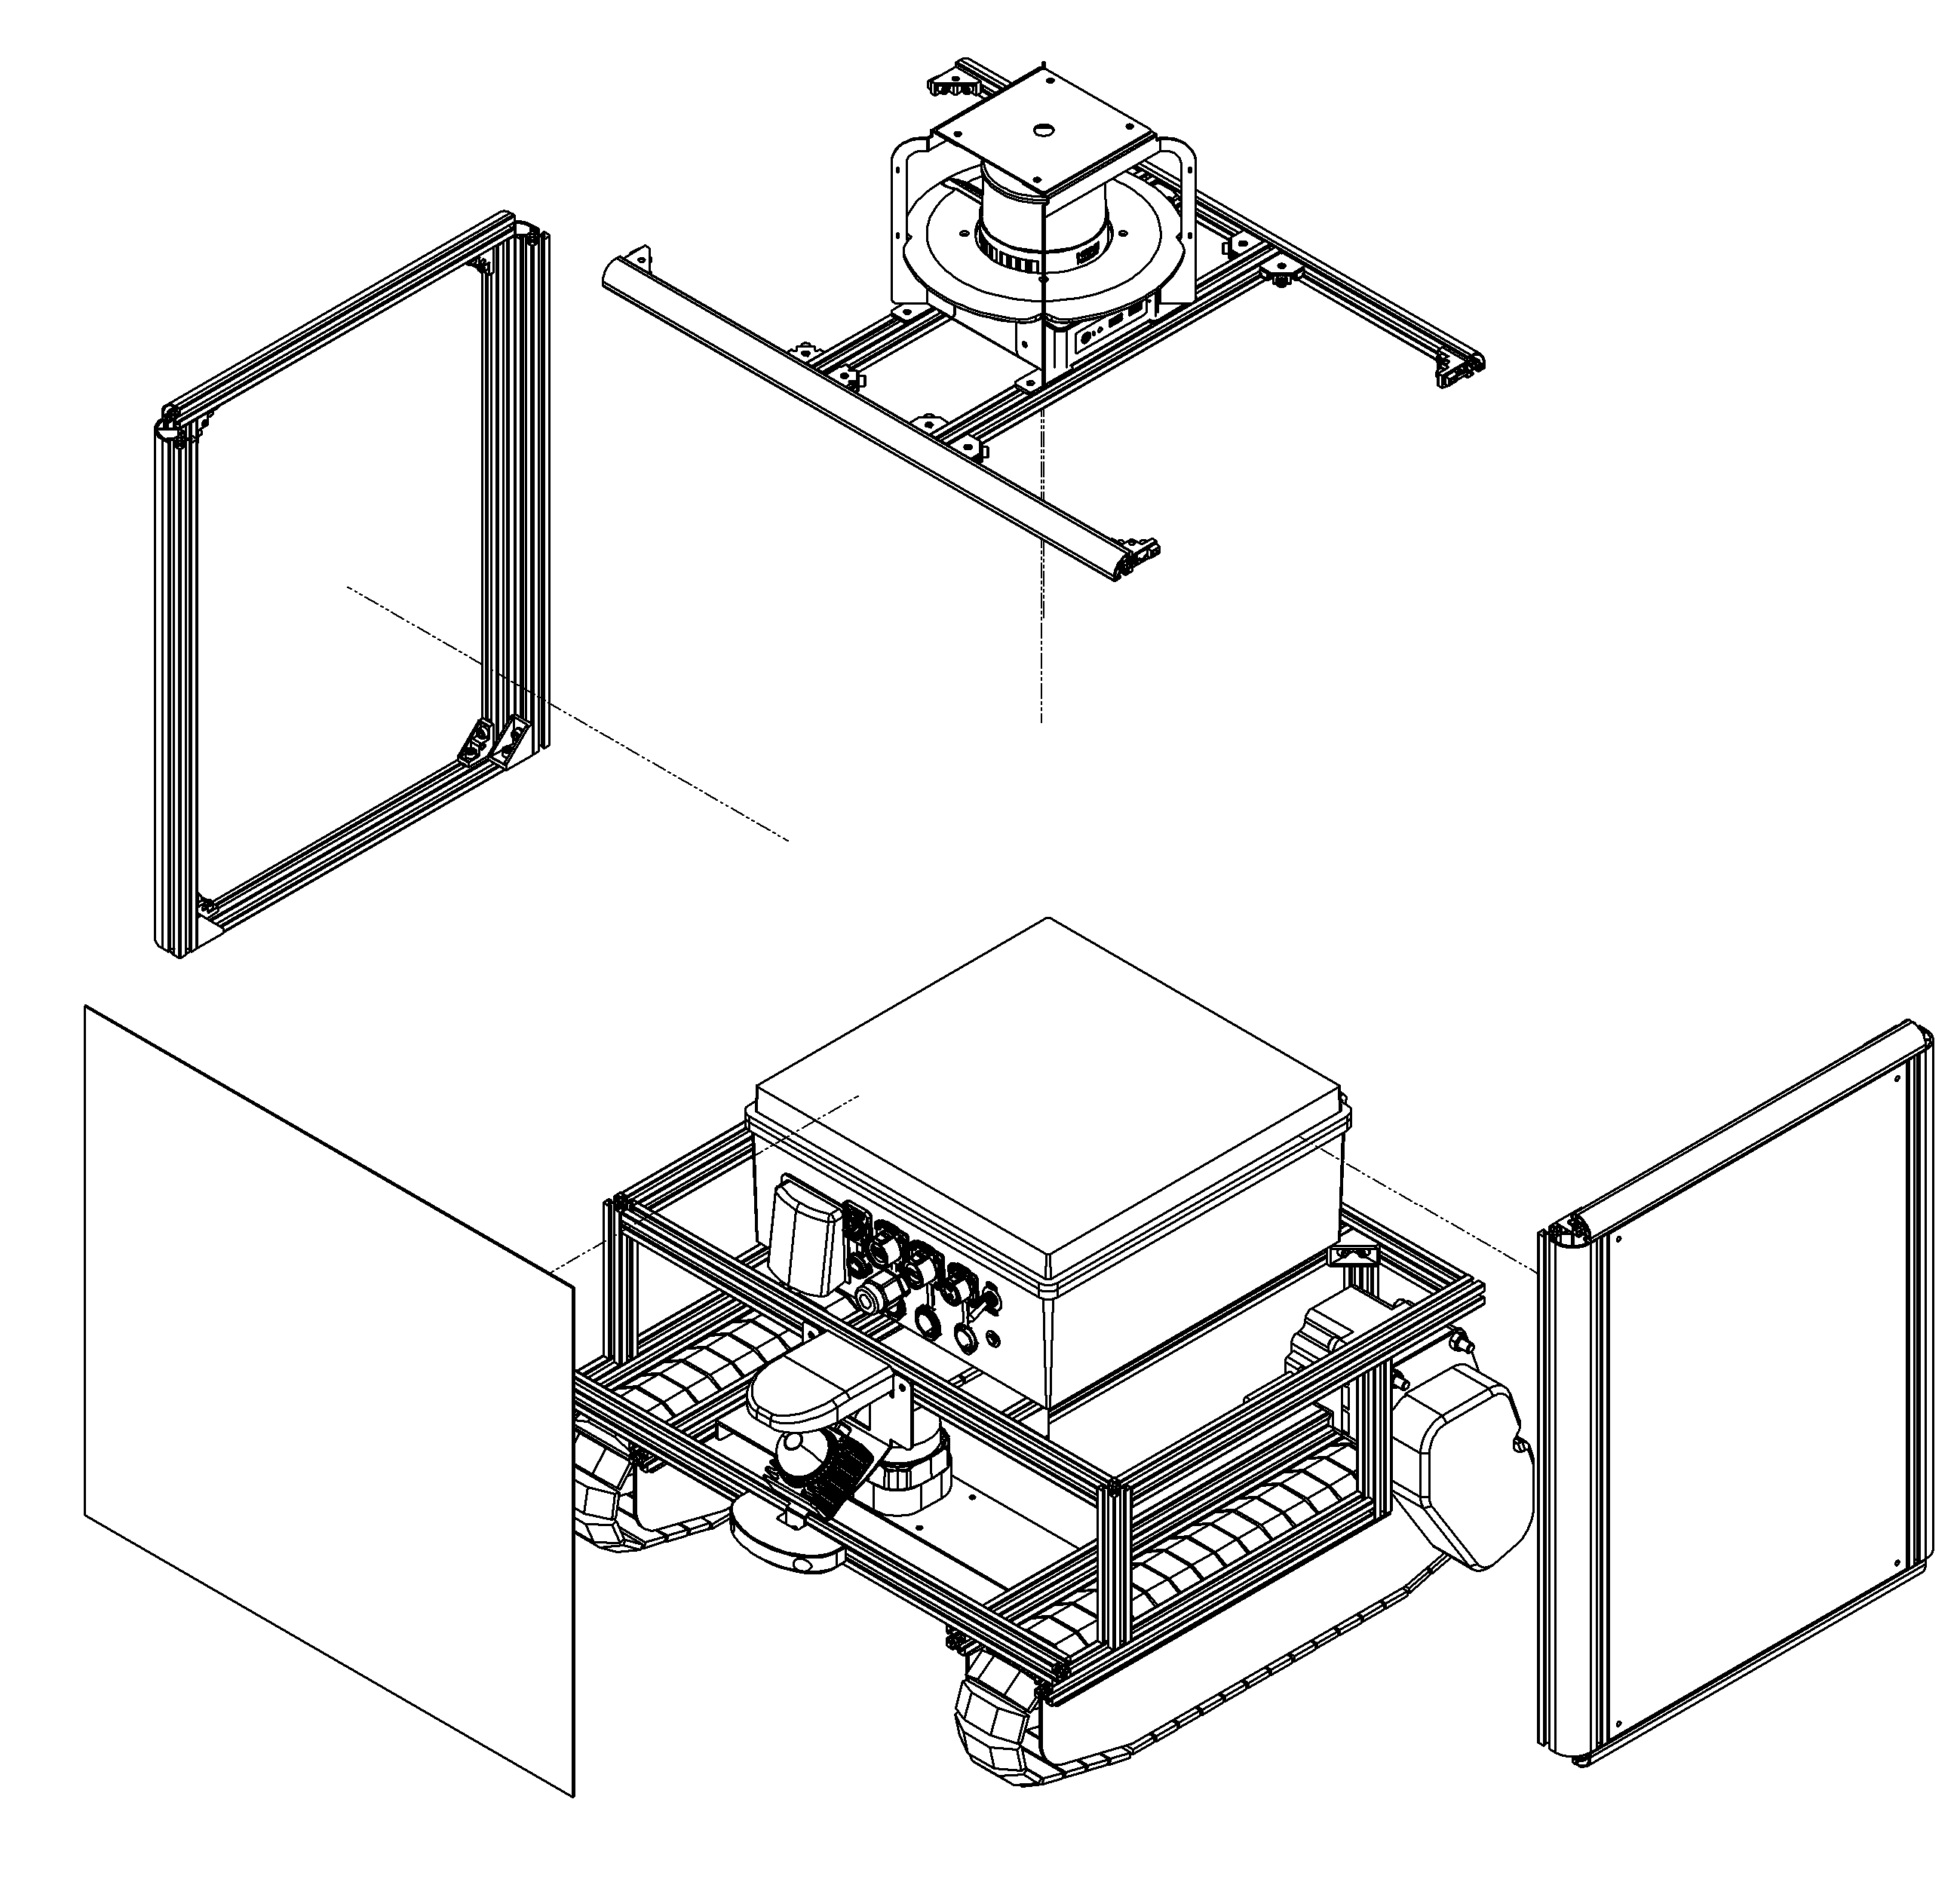
\includegraphics[width=\hsize]{fig/exploded_view.png}
       \caption{右の図}
       \label{fig:migi}
    \end{minipage}
  \end{figure*}
\section{システム}


\subsection{ハードウェア}
自律走行を行う機体で必要な要素は大きく分けると下記5点となる。

\begin{itemize}
    \item センサ
    \item 走行装置
    \item 計算機
    \item バッテリー
    \item シャーシ
\end{itemize}

この章では、搭載したハードウェアがどのように使用されたか説明する。

\subsubsection{自律走行ロボット:Penguin}
今回、自律走行を実現する基本的な構成を持ちつつ、不整地の走行も可能な機体とすることをコンセプトに、機体を作成した。 
作成した機体とその搭載した機器を、図nに記載する。この章では、各要素について詳細を説明する。

\subsubsection{センサ}
Penguinには、オドメータ、IMU、LiDARの3種類のセンサが搭載されている。

オドメータはモータの回転数を計測するもので、どのくらいモータが回転したか累積を数えることでロボットのホイールオドメトリを推定する。
ただし、スリップや量子化誤差などで誤差が蓄積するためこの値をそのまま使用することはできない。
後述のLiDARを使って外界の情報を得ることで補正して使用した。

IMUはロボットのX,Y,Z方向の加速度とRoll、Pitch、Yaw方向の角加速度を取得できる。
この値を累積することで、ジャイロオドメトリを推定することができる。
ホイールオドメトリのようにスリップすることはないが、段差などの影響を強く受ける。
今回は、SLAMアルゴリズムでの位置補正に使用した。

LiDARは距離を知ることができるセンサである。
今回搭載したLiDARは3DLiDARで、ロボット周辺の形状を3次元の点群として得ることができる。
3DLiDARは自己位置推定用のものと、障害物認識用のものの2つを搭載した。

自己位置推定を行うためのLiDARセンサとして、Velodyne社のVLP-16\cite{VLP16}を搭載した。
VLP-16は100mという長距離の測定が可能であるため、つくば市庁舎やつくばエクスプレスの建物を常に観測できる。
ロボット近傍で人だかりができて周囲の景気が見えづらくなっても、自己位置推定を維持しやすい。
なるべく周囲の物体によってLiDARの光を阻害されないように機体の最上部に搭載した。
また、非常に高額なセンサであるため、転倒したり、ものが当たって傷つかないように金蔵製のガードも合わせて設置した。

障害物を検出するLiDARとして、Livox社のMID-360\cite{MID360}を搭載した。
MID-360はVLP-16のような長距離の物体を測定することはできないが、非常に密な空間測距ができる。
また、FoVも60度と広く、ロボットに衝突しそうな近くの物体を精細に取られることができるLiDARである。

障害物検知用のLiDARは、接近する物体を検知するため、機体の下部に設置し、35度下向きに傾けて設置した。
これにより、ロボットの前方250mmの地面を測距できるため、衝突しそうになるギリギリまでの距離の物体を測定できる。
また、今回の機体は後進を行わないため、障害物の検出範囲は前方向のみとした。
障害物検出用のLiDARも、光学窓への傷を防ぐため金属製のガードを上下に設置した。

\subsubsection{走行装置}
走行装置には、CuboRex社のクローラロボット開発プラットフォーム CuGo V4\cite{CuGo}を使用した。
不整地走行に適したクローラを有するプラットフォームを使用する事で、不整地の走破性向上と開発の高速化を図った。

\subsubsection{計算機}
ロボットの制御を行うPCとして、ASUS社のROG Strix SCAR 15 G532LWS\cite{PC}を搭載した。
ノートPCを搭載することにより、ロボットを駆動する電源系列とPCを駆動する計算機の電源分割を実現した。

モータの制御には、CuboRex社製モータドライバに付属しているRaspberry Pi Pico\cite{PICO}を使用した。

\subsubsection{バッテリー}
機体下部に、24V20Ah のLiFePO4バッテリを搭載した。
本機体は不整地走行の可能性を考慮し、LiPoバッテリより安全性の高いLiFePO4バッテリーを採用した。

バッテリは機体下部に設置することで、重心の上昇による安定性の低下を防いだ。
バッテリから供給される電源は、ロボットに搭載した電源分配基板により適切に切替・分配・変圧し、PCを除く各機器に接続した。

\subsubsection{シャーシ}
屋外でのデバッグ作業を想定し、日よけの壁を搭載した。
ロボットは図nのような5ユニットで構成し、各部を計10本のボルトで分解できる形とした。
分解箇所には付当てを設置し、複数回の分割、組立を実施しても再現性のあるシャーシとなる形とした。

構造部材にはミスミ社 R形状アルミフレーム\cite{MISUMI}を使用することで、衝突しても対象に危害を加えにくい形状を実現した。
突起部・巻き込みが発生しうる箇所には、樹脂製のカバーを搭載した。

ロボットの状態表示のため、アルミフレームの溝部にLEDを搭載した。
このLEDの色でロボットが自律走行状態か、操作者による操作を実施している状態かを一般通行者に対して示した。

\begin{figure*}[H]
    \centering
    \begin{minipage}[b]{0.45\hsize}
       \centering
       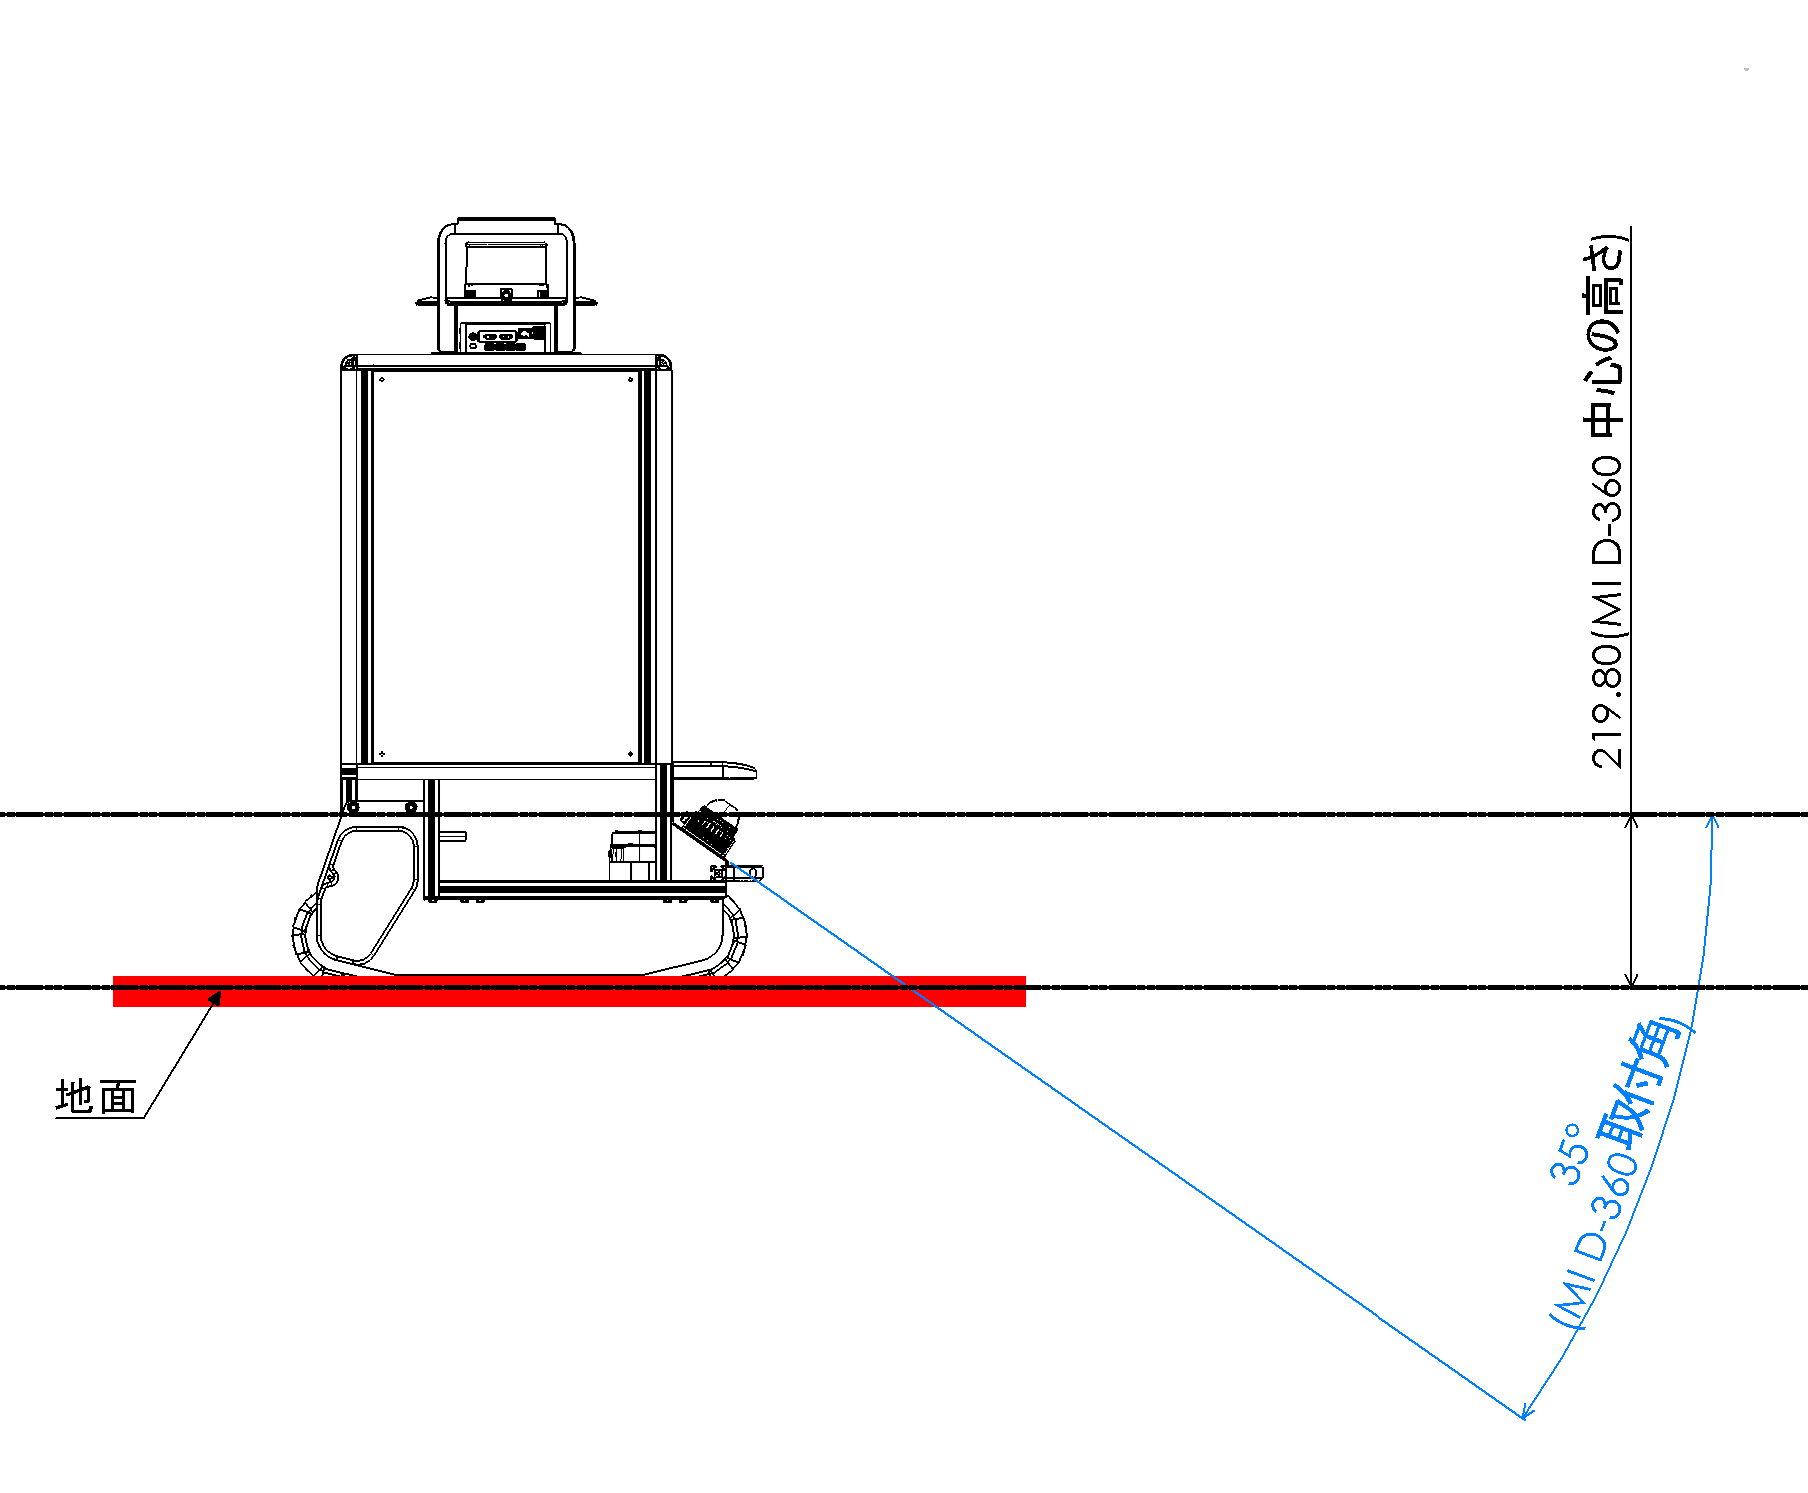
\includegraphics[height=5cm]{fig/obstacle_detection_range_sideview.png}
       \caption{左の図}
       \label{fig:detection}
    \end{minipage}
  %
    \begin{minipage}[b]{0.45\hsize}
       \centering
       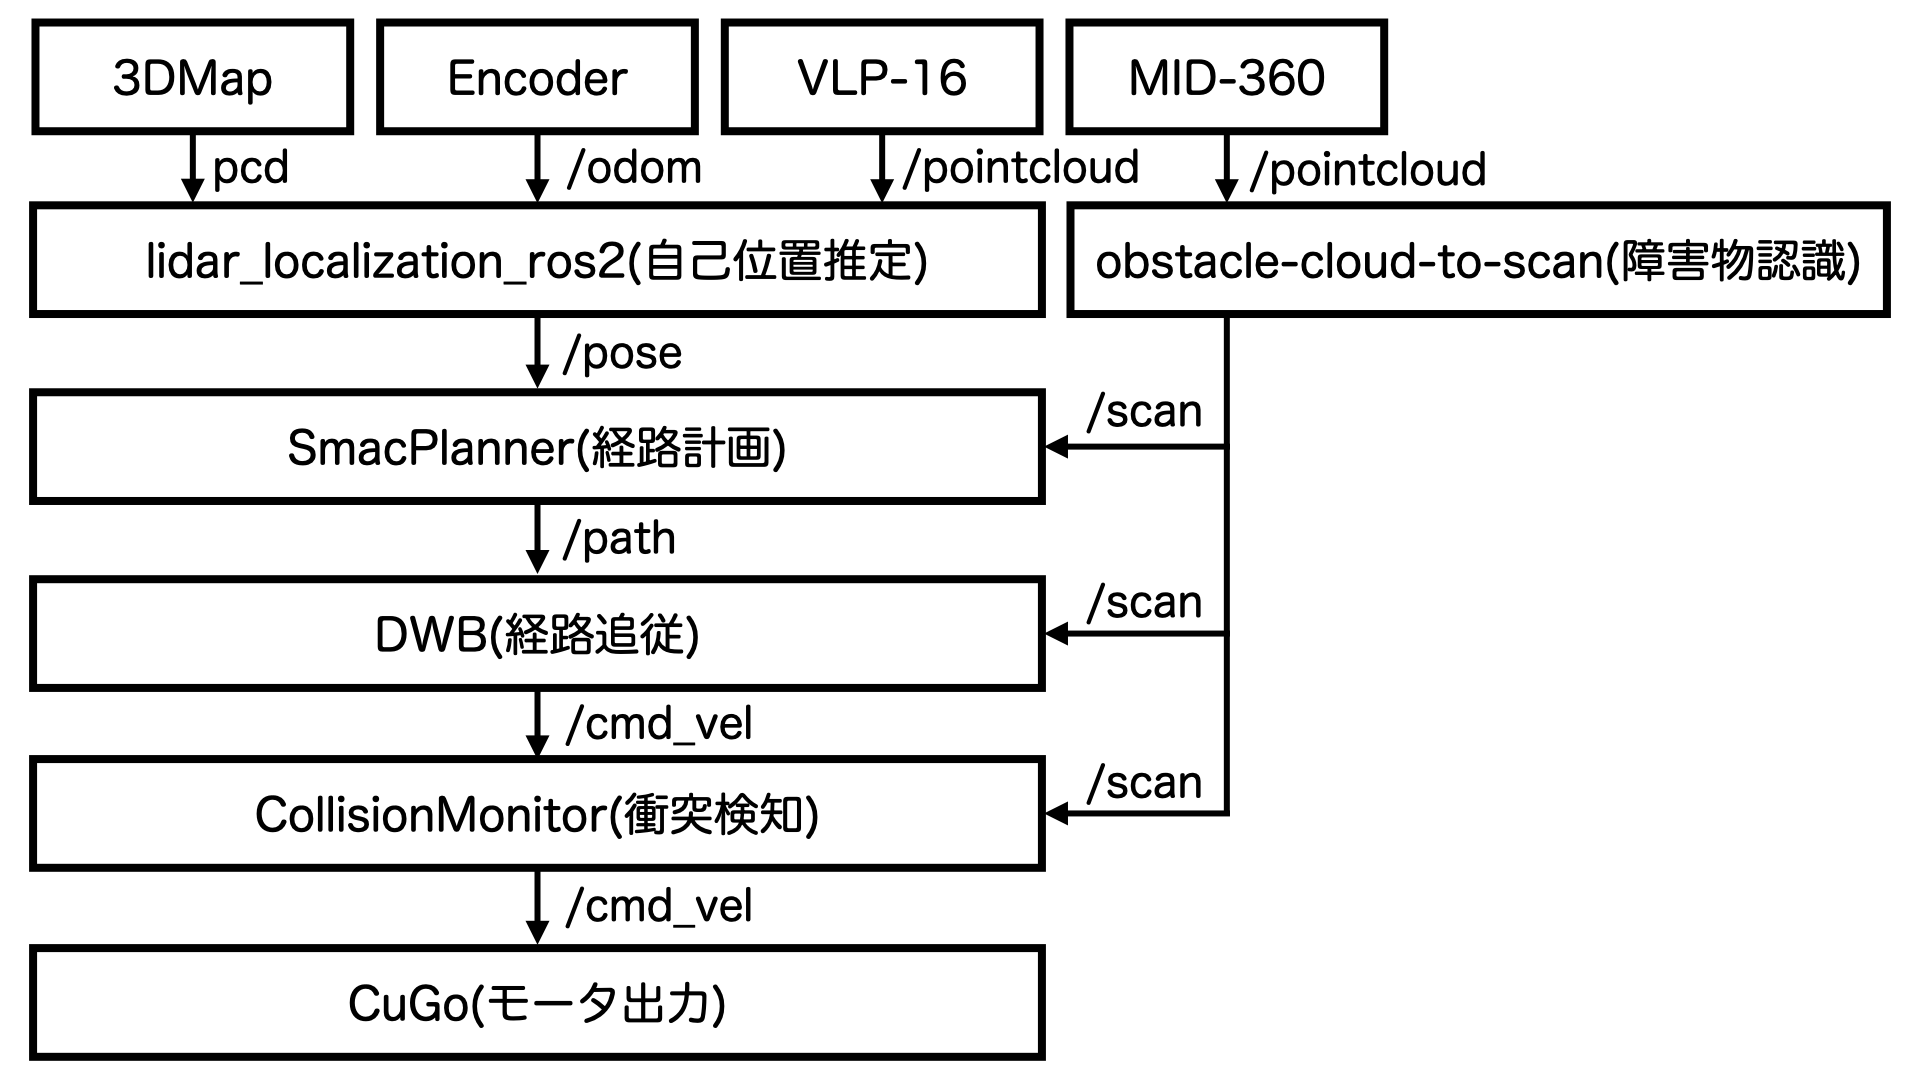
\includegraphics[height=5cm]{fig/system.png}
       \caption{ナビゲーションシステムの構成}
       \label{fig:system}
    \end{minipage}
\end{figure*}

\subsection{ソフトウェア}
ロボットを走行させるためのソフトウェア構成は以下の通りである。
\begin{itemize}
    \item 地図作成
    \item 自己位置推定
    \item 障害物認識
    \item 経路計画
    \item 経路追従
\end{itemize}

自律走行を実現するために、上記のタスクを同時に満たすシステムを構築した。
図nにソフトウェアシステムの概要を示す。
このシステムを構築するために多くはOSSであるROS 2\cite{ROS2}を使用した。
このレポートでは、上記のそれぞれのタスクについてどのようなアプローチをしたか述べる。

本システムで自律走行をするためには走行する範囲の地図を作成する。
現実の場所とリンクした地図をロボットに持たせることでロボットが目的地と現在地の相対位置把握することができる。
このロボットに持たせる地図の精度が後述の自己位置推定の精度に大きな影響を与えるため、効率的で精度の高い地図を作成することが大事である。
この地図作成は第3章で説明する。

次に、ロボットの現在位置を推定する。LiDARなどのセンサ情報から自分自身が地図上のどの位置にいるのかを推定する。
現在位置が分かれば、目的までの向かう経路を計算することができる。
正確な位置情報を維持し続けるために3Dの地図から回転式3DLiDARのセンサ値とオドメトリ情報を使用して自己位置推定を行う方法を第4章で説明する。

自己位置推定ができても、実際には障害物があってたどり着かないことがほとんどである。
向かいたい場所までの経路上に障害物がどのようにあるのか反映させる。
ロボット直近の広範囲で高密度な点群を取得できる3DLiDARを使用して、2DLiDARでは見逃しがちな細長い物体を検知し、坂道などの検知したくない物体を除外することができた。
この障害物検知手法は第5章で説明する。

ロボットの現在位置と障害物を知ることができると、目的地までの障害物を避けた経路を計算することができる。
実際の自律走行では、スタート地点から本走行のゴール地点まで1度に経路を計算しない。
数メートルおきに小さなゴール地点を作成し、そこに到達することを繰り返す。
経路を計算した後には、ロボットがこの経路を正確にトレースするようにアクチュエータの出力を制御する。
しかし、線路の上を電車が走行するように、計算した経路を忠実に走行すれば良いとは言えない。
ロボットハードの都合で急停止や急旋回が物理的に実現できなかったり、とっさに現れた障害物を回避する必要があるためである。
障害物を回避しながら、必要十分に経路をなぞる制御を経路追従という。
第6章では、経路計画と経路追従を行うナビゲーションについて説明する。

最後に、本走行の結果と今後の展開について述べる。
\begin{figure*}[htbp]
    \centering
    \begin{minipage}[b]{0.45\hsize}
       \centering
       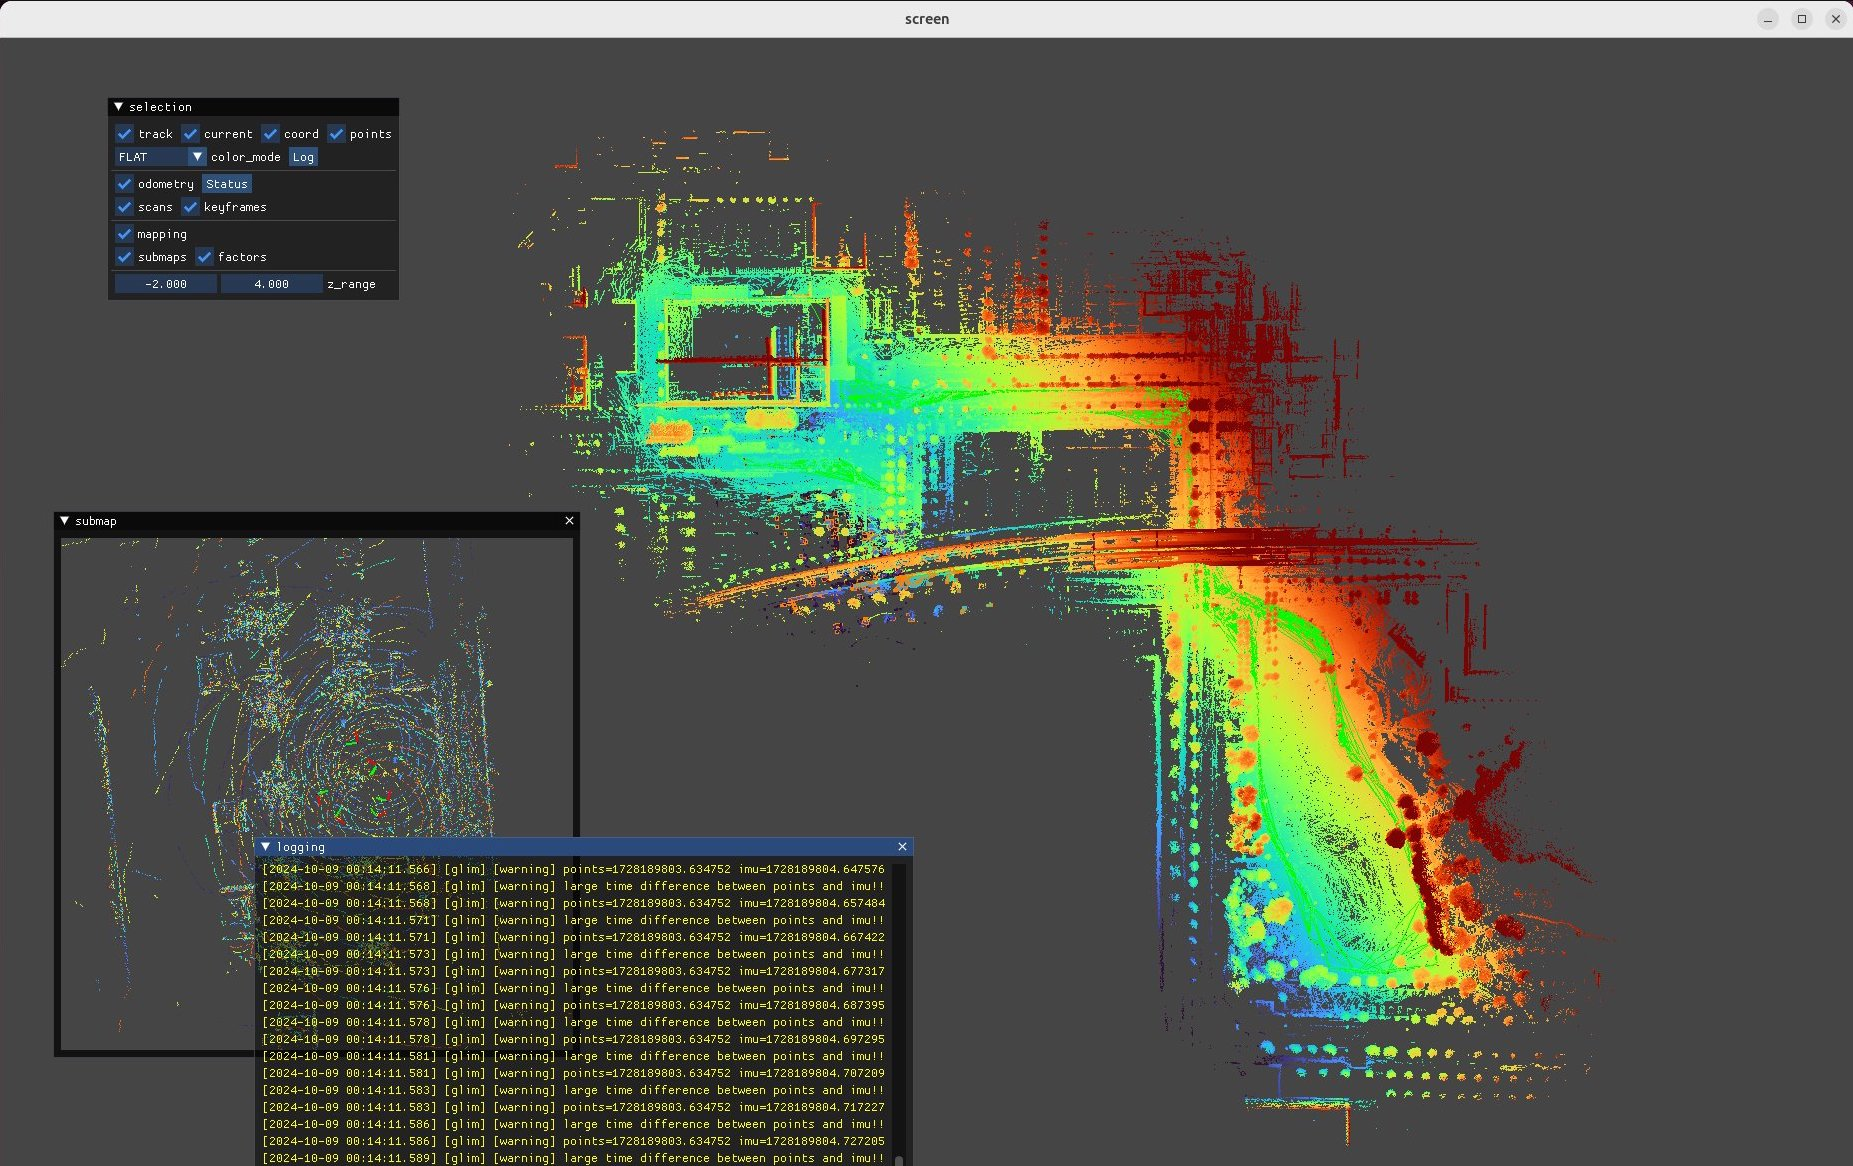
\includegraphics[height=5cm]{fig/tsukuba_map.jpeg}
       \caption{作成した3D地図}
       \label{fig:tsukuba_map}
    \end{minipage}
  %
    \begin{minipage}[b]{0.45\hsize}
       \centering
       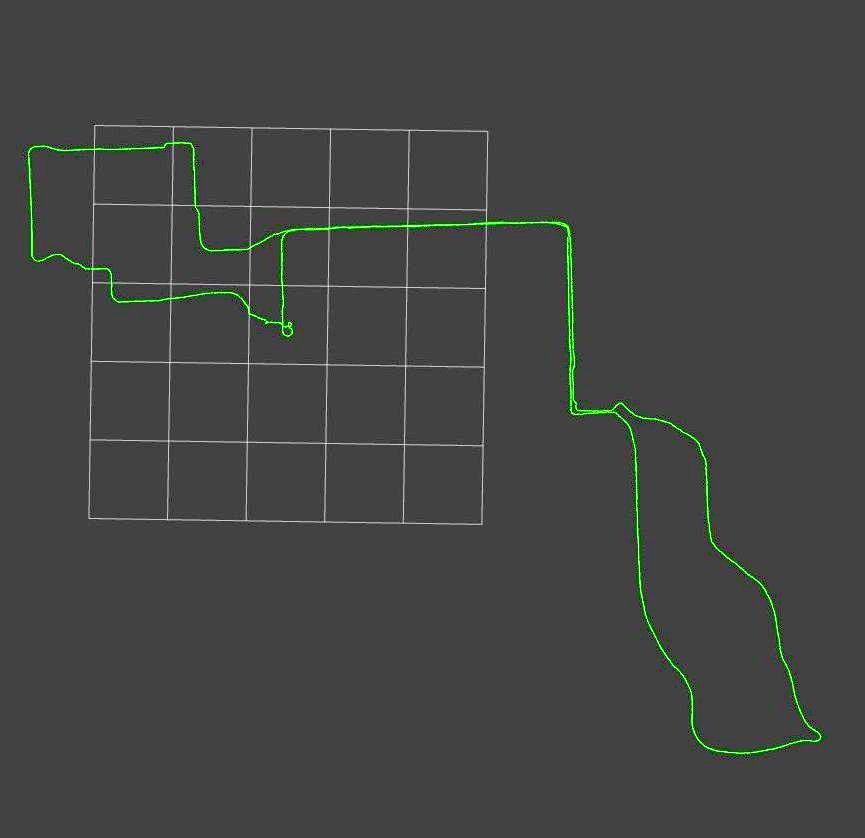
\includegraphics[height=5cm]{fig/trajectry.jpeg}
       \caption{自己位置推定した軌跡}
       \label{fig:trajectry}
    \end{minipage}
  \end{figure*}
\section{地図作成}
現代の多くの自律走行ロボットは、行動範囲分の環境地図を必要とする。
ロボットが環境地図を持つことにより、既知の環境内で自由に行動することを目指す。

物流倉庫やオフィスビルなどの環境では2Dの地図を使用しても充分に効果を発揮する。
しかし、つくばチャレンジのようなひらけた場所であったり、交通の往来があったりする屋外環境であると2D地図の使い方によっては、性能が不十分になることがある。
このつくばチャレンジ2024では、回転式3DLiDARを利用し3D地図を作成した。
3D地図は複雑な環境や、本走行のように人だかりでロボット周辺に障害物がたくさんあってもロバストに自己位置推定を続けることができた。
回転式3DLiDARは非常に高価であるが、つくばチャレンジでは、無料貸与があるため、参加者は利用できるチャンスがある。
つくばチャレンジ2024では、株式会社アルゴさまより無料で貸与いただいた。
ここにお礼のことば(謝辞行きかどうかは要検討)

\subsection{GLIM}
地図作成には、回転式3DLiDARで、GLIM\cite{GLIM}を用いて作成した。
GLIMはさまざまな3DLiDARに対応したSLAM手法である。
IMUやオドメトリを入力することでLiDARの値とタイトカップリングで位置推定するため、より正確なSLAMを行うことができる。
3DLiDARの回転式やソリッドステート式だけでなく、深度付きカメラにも対応する。
IMUやオドメトリの有無も選ぶことができるため、利用の敷居はとても低い。

作成したつくばチャレンジの走行範囲全域の地図は図nの通りである。
つくばチャレンジの現場でロボットのセンサを起動し、スタート地点からゴールまで走行した時のセンサデータを入力し作成した。

\subsection{パラメータチューニング}
GLIMのチューニングとしては以下の点を変更した。
\begin{itemize}
    \item k\_correspondences
    \item voxel\_resolution
\end{itemize}

k\_correspondencesは一つのサブマップを構築する際に利用する点群のスキャンの数である。
回転式LiDARの16ラインのものだと点群が疎であるため、この数を上げないとマッチングに必要な点群数に至らないことがある。
32ラインのLiDARはデフォルトから変更なし、16ラインのLiDARは数を30程度に設定するとうまく地図が構築されることを確認した。

voxel\_resolutionは3次元空間の点群を配置する解像度である。
つくばチャレンジ2024のようなキロメートルオーダーでは、デフォルトの0.1m四方だと、GPUメモリ8GBが飽和した。
今回は0.25m四方に設定したら、研究学園駅前公園を含むすべての範囲で地図を作成することができた。

最後にGLIMのオフラインツールで追加でループクローズを設定する。
SLAMを実施した後、オフラインツールで再度開くと、各サブマップ同士の位置関係をグラフィカルに確認することができる。
このツールで、スタート地点、往路と復路が重なるパイロン地帯、横断歩道の待機場所で再度ループクローズをかけることで、より正確な地図に修正された。

これらの作業を通じて、つくばチャレンジ全域で自己位置推定ができる地図ができた。
つくばの3D地図はGoogleDriveの\url{https://x.gd/22GO4}で公開しているので、来年同じ構成で使用したい方は使うと良い。
\section{参考文献}
参考文献の参照例.
\begin{itemize}
\item 論文誌の参照例 \cite{Article_01}
\item 本の参照例 \cite{Book_02}
\item 国際会議の参照例 \cite{Inproc_03}
\item 技術報告の参照例 \cite{Techrep_05}
\item Webページの参照例 \cite{Web_06}
\end{itemize}
\section{障害物認識}
自己位置とゴールが分かればロボットが進むべき経路を計算できる。
ただし、これだけでは現実にある衝突してはいけない障害物を考慮していない。
LiDARなどのセンサを使って障害物を認識し、それを地図に反映させることで障害物を考慮した経路を計算できる。
多くのロボットでは、2DLiDARを障害物に使用している。
2DLiDARを使うと坂道など地面が写ってしまう。
2DLiDARを使うと机のような物体は脚しか映らない。
3DLiDARを使うことで机の柱と天板の部分の全体の点群を得ることができる。
2DLiDARと異なり、ぶつかりたくない部分を抽出して点群として表現できる。
メカの章に載せた、MID360でを使用した。
これを実現するROSパッケージを作成した。
簡単な手順としては以下の通りだ。
点群をダウンサンプリングする。
LiDAR点群の傾きを設置角度から逆算して水平にする。
法線を各点ごとに計算する。
法線ベクトルから水平なものは地面など問題ないものと判断した。
法線ベクトルから垂直に近いものは壁や障害物と判断した。
計算を単純にするために、法線のZ方向で閾値で区切った。
これで坂道や乗り越え可能な5cm程度の小物は水平と判断し障害物判定できた。
細い鉄パイプやパイロンの根本も障害物として判定できた。
出力した点群をOSSのPointCloudToLaserScanパッケージに入力し、2DLiDARのscanトピックに変換した。
このScanトピックをNavigation2に入力することで、広く使われる2DLiDARのサンプルをそのまま動かすことができた。
つくばチャレンジ環境で使用してパイロンや人、生垣などの大半の障害物を検出することができた。
パイロンは先端の細いところから根本の一番太いところまで観測できた。
この方式では、パイロンの一番太いところをScanとして出力するため、パイロンのぎりぎりを通過することがすくない。
苦手な物体として、背のひくい水平な障害物は検出することが難しい。
平台車。
小さな段ボール。
地面成分が大きく平均化され溶け込んでしまう。
2.4GHz CPUシングルスレッドで40msくらい。
8スレッドで分散処理して7msくらい。
PCの電飾消費が深刻だったので、あえてシングルスレッドの実装で走行した。
パッケージはOSSで公開しているので、ぜひ利用してほしい。
\section{ナビゲーション}
ROS 2では、自己位置推定、経路計画、経路追従の手法が詰め合わせとなっているパッケージとしてNavigation2\cite{macenski2020marathon2}がある。
このNavigation2パッケージを利用することで、それぞれのタスクを処理するアルゴリズムを利用できる。
今回は3次元地図で自己位置推定を行なっているので、経路計画と経路追従のアルゴリズムを利用した。

\subsection{経路計画}
経路計画は現在の位置座標からゴールとなる座標までの区間でロボットが到達可能な経路を計算するタスクである。
経路計画は2次元の占有格子地図上で計算した。
ロボットに持たせている3D地図は、単純に地図上の座標を知ることのみで利用している。
この3次元の自己位置座標から、2次元空間で利用するために、X,Y,Yawの値をそのままコピーするだけで2Dに転写した。

経路計画を行う時は、いきなり最終目的地への経路を計画するのではなく、
数メートルおきに小さなゴールを用意し、到達したらまた次の小さなゴールに向かって経路計画を行う。
この小さなゴールをWaypointと呼ぶ。

Waypointをロボットの状況に合わせて通知するPenguin\_navパッケージ\cite{Penguin}を作成した。
Penguin\_navは...

Penguin\_navから受け取ったWaypointまでの経路を計算する。
Navigation2では、さまざまな経路計画アルゴリズムを利用することができる。
今回はSmacPlanner\cite{macenski2024smac}を利用した。
SmacPlannerはNavigation2のPluginに実装されているため、ConfigファイルでSmacPlannerを選択するだけで利用できる。

SmacPlannerはロボットの形状を考慮した衝突判定をしてくれる。
したがって、自ロボットの投影面積であるポリゴンを指定するだけで、無茶な経路は選ばれなくなる。
また、最小回転半径も指定できるため、なめらかな円弧で走行経路を利用できる。
クローラは非常に抵抗が大きく、その場旋回がとても大変な駆動方法である。
そのため、最小半径を0.4mに設定した。
これにより、走り出しのぎこちなさを抑えつつも、必要に応じて急旋回もできる曲率となった。

\subsection{経路追従}
前節のSmacPlannerで計算された経路をロボットがどのように再現するか計算するアルゴリズムを経路追従アルゴリズムという
Navigation2では、さまざまな経路追従アルゴリズムを利用できる
つくばチャレンジ2024では、DWBをつかった
DWBはロボットが再現可能な速度や加速度の範囲の中で一番良い速度を選択する
最高速度と最低速度と加速度を設定できる
クローラの制御の場合、抵抗が非常に大きく初動に大きなエネルギーを必要とする
最低速度を速く設定し、すぐに停止できるように減速加速度を大きくなるように設定した。
\begin{figure*}[h]
    \centering
    \begin{minipage}[b]{0.45\hsize}
       \centering
       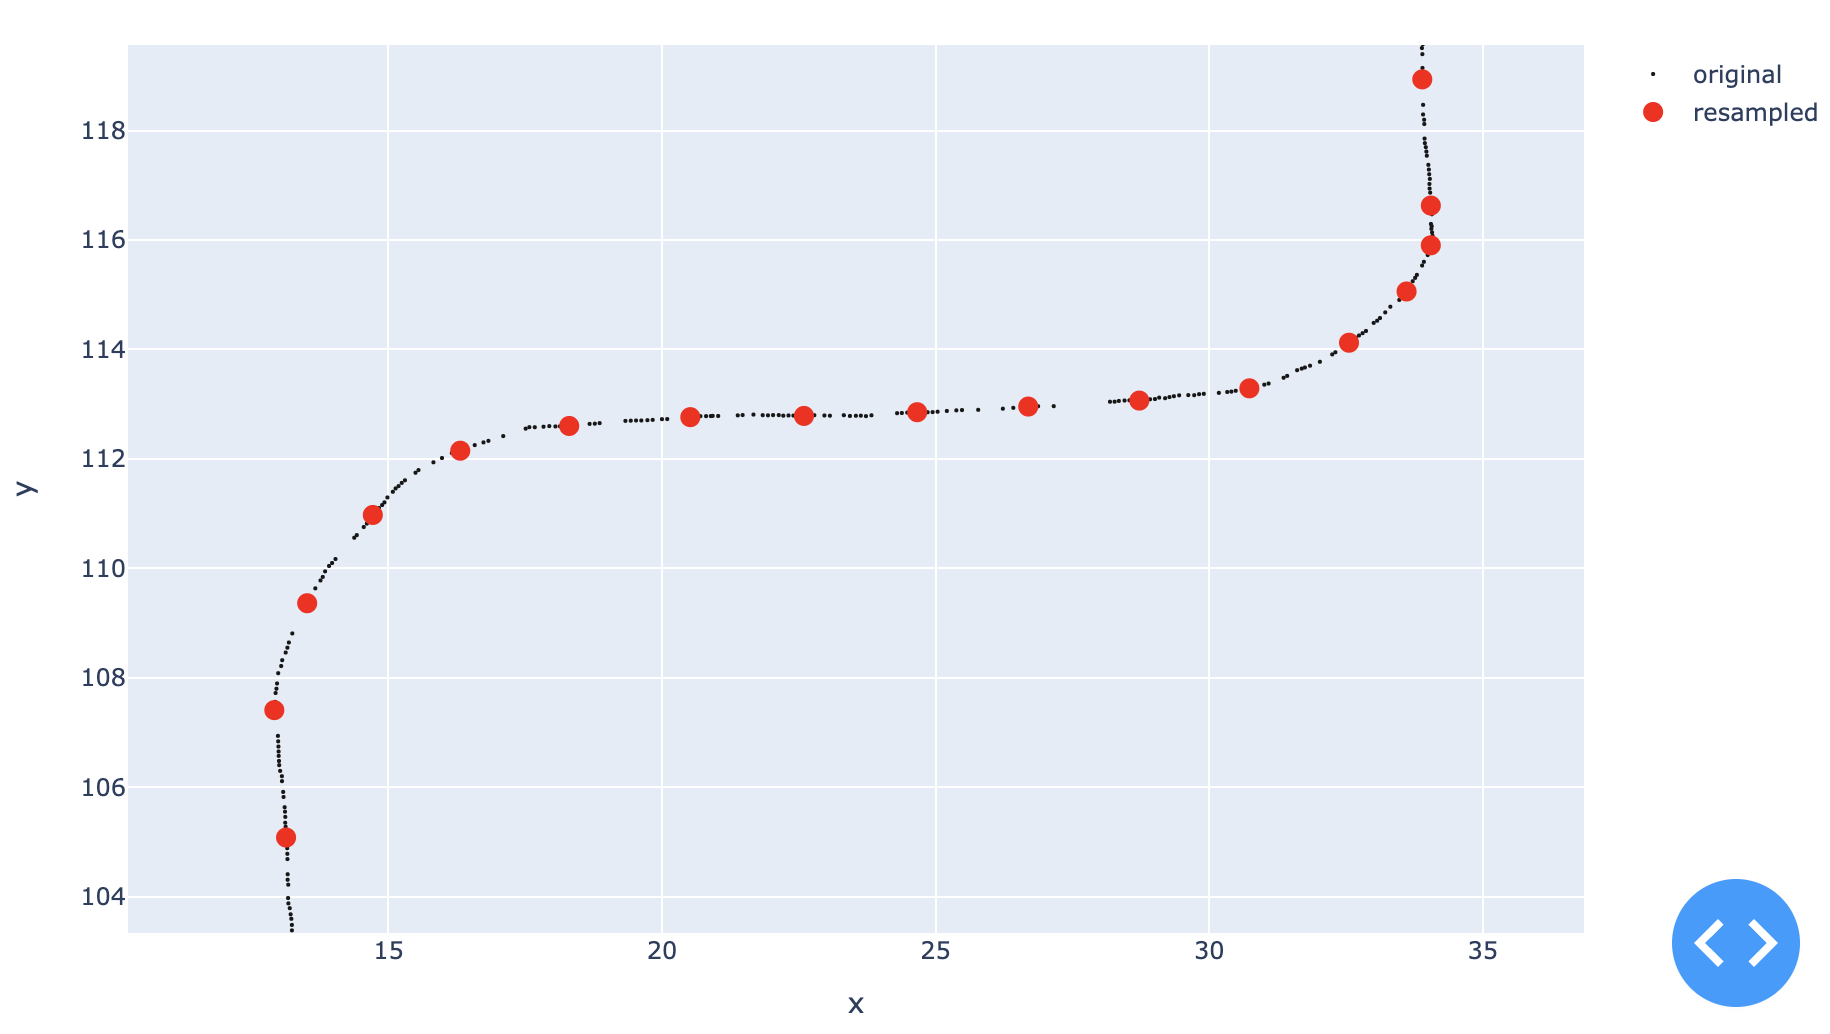
\includegraphics[width=\linewidth]{fig/waypoint_resampler.png}
       \caption{waypoint\_resamplerによりダウンサンプリング。黒点が入力の自己位置推定結果で、赤点がダウンサンプリングした点列}
       \label{fig:waypoint-resampler}
    \end{minipage}
  %
    \begin{minipage}[b]{0.45\hsize}
       \centering
       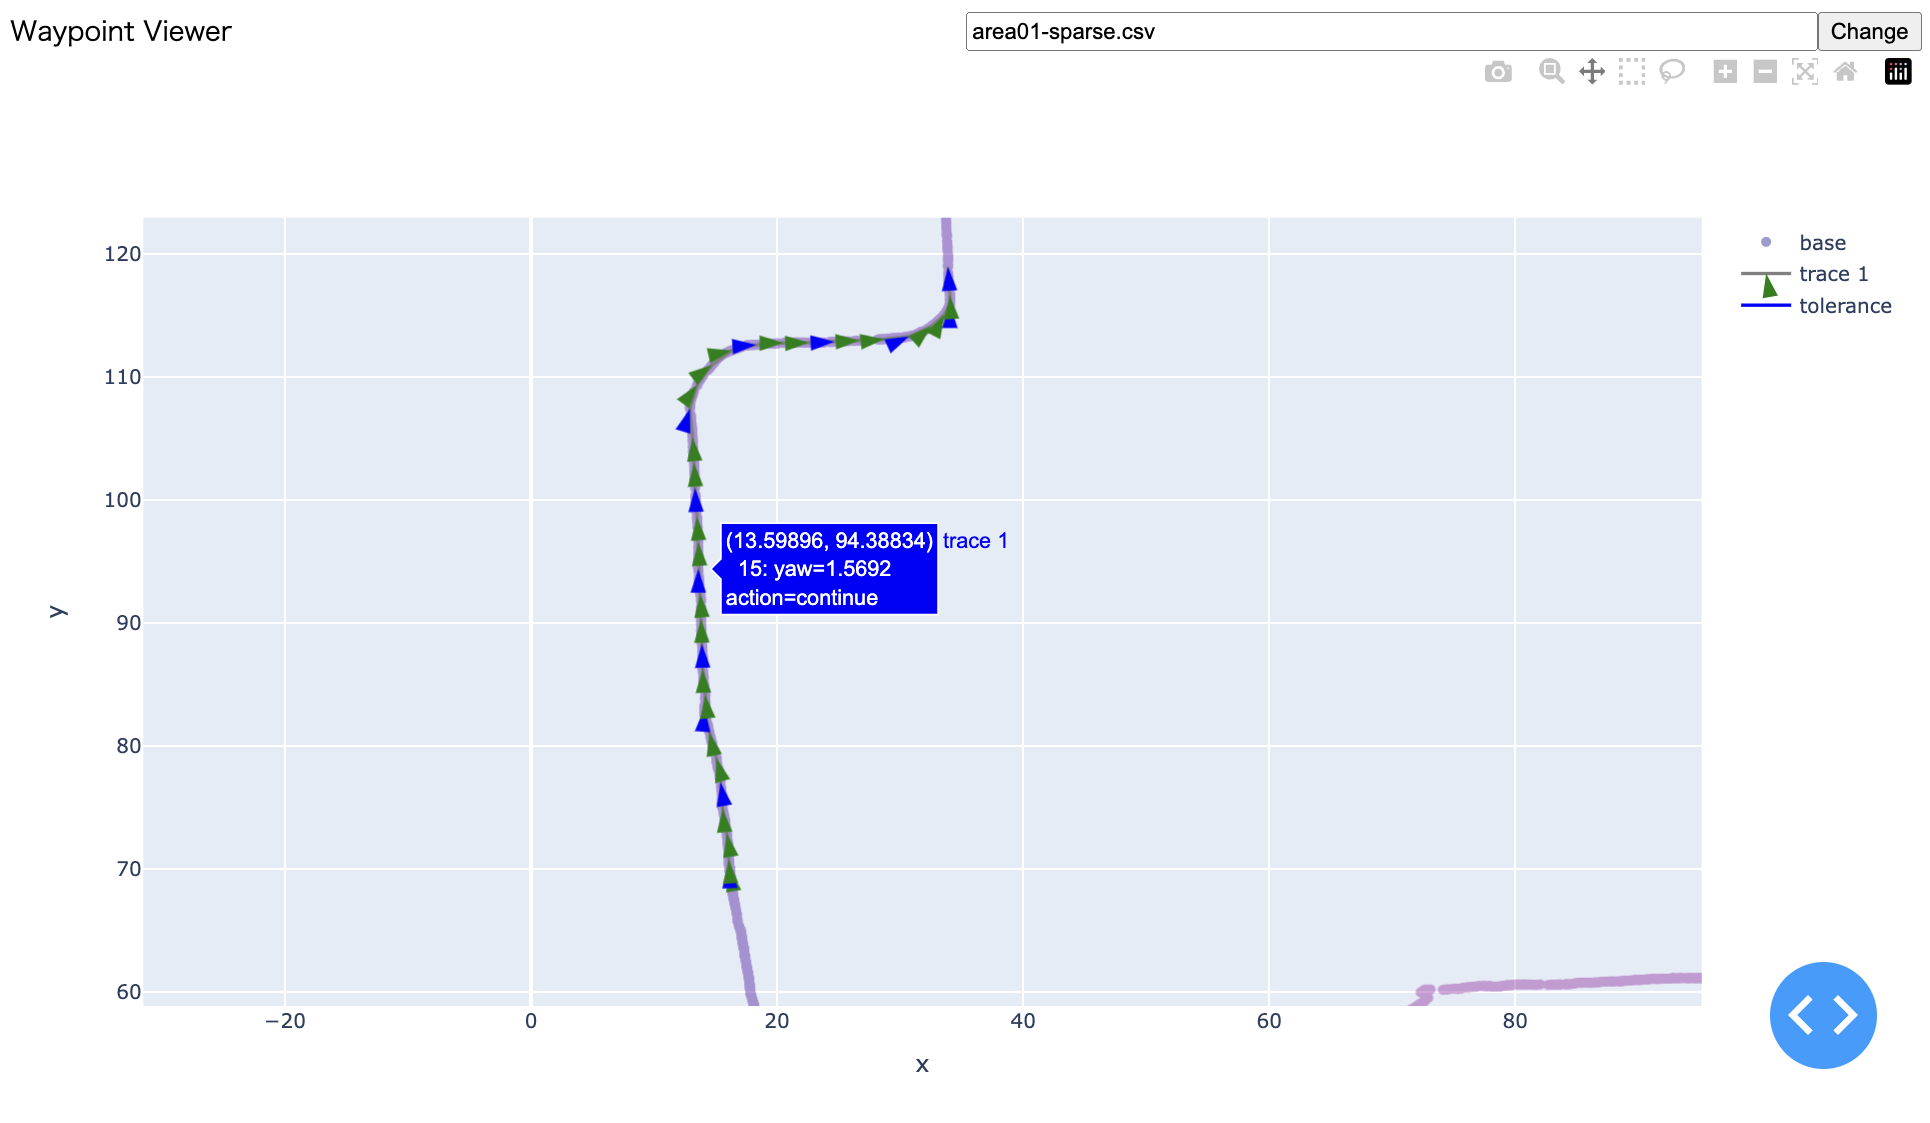
\includegraphics[width=\linewidth]{fig/waypoint_viewer.png}
       \caption{waypoint\_viewer。左の画面は外部のCSVエディタ}
       \label{fig:waypoint-viewer}
    \end{minipage}
\end{figure*}

\begin{figure*}[bhtp]
    \centering
    \begin{tabular}{cc}
        \begin{minipage}[b]{0.45\hsize}
        \centering
        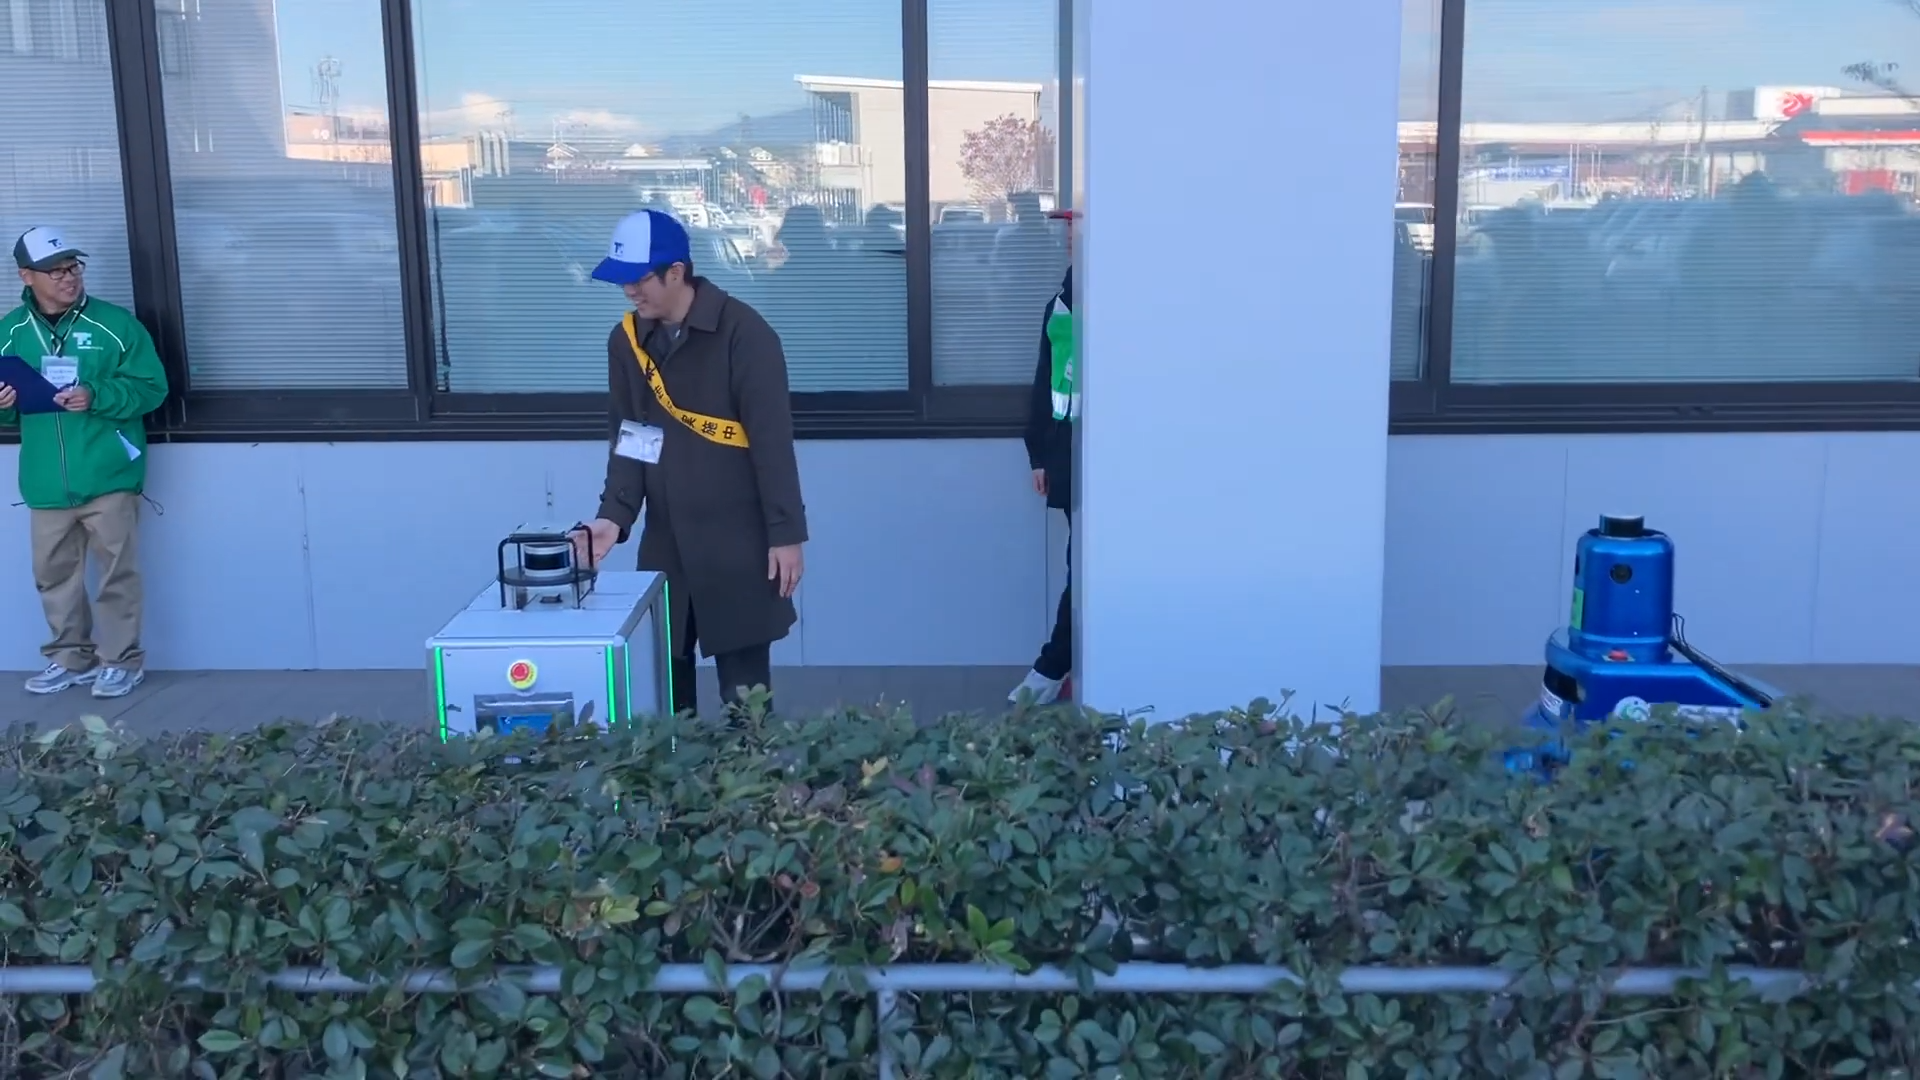
\includegraphics[width=\linewidth]{fig/honsoukou1.png}
        \caption{狭路走行中、走行と停止を繰り返した。後続のロボットが渋滞となってしまった}
        \label{fig:honsoukou1}
        \end{minipage} &
    %
        \begin{minipage}[b]{0.45\hsize}
        \centering
        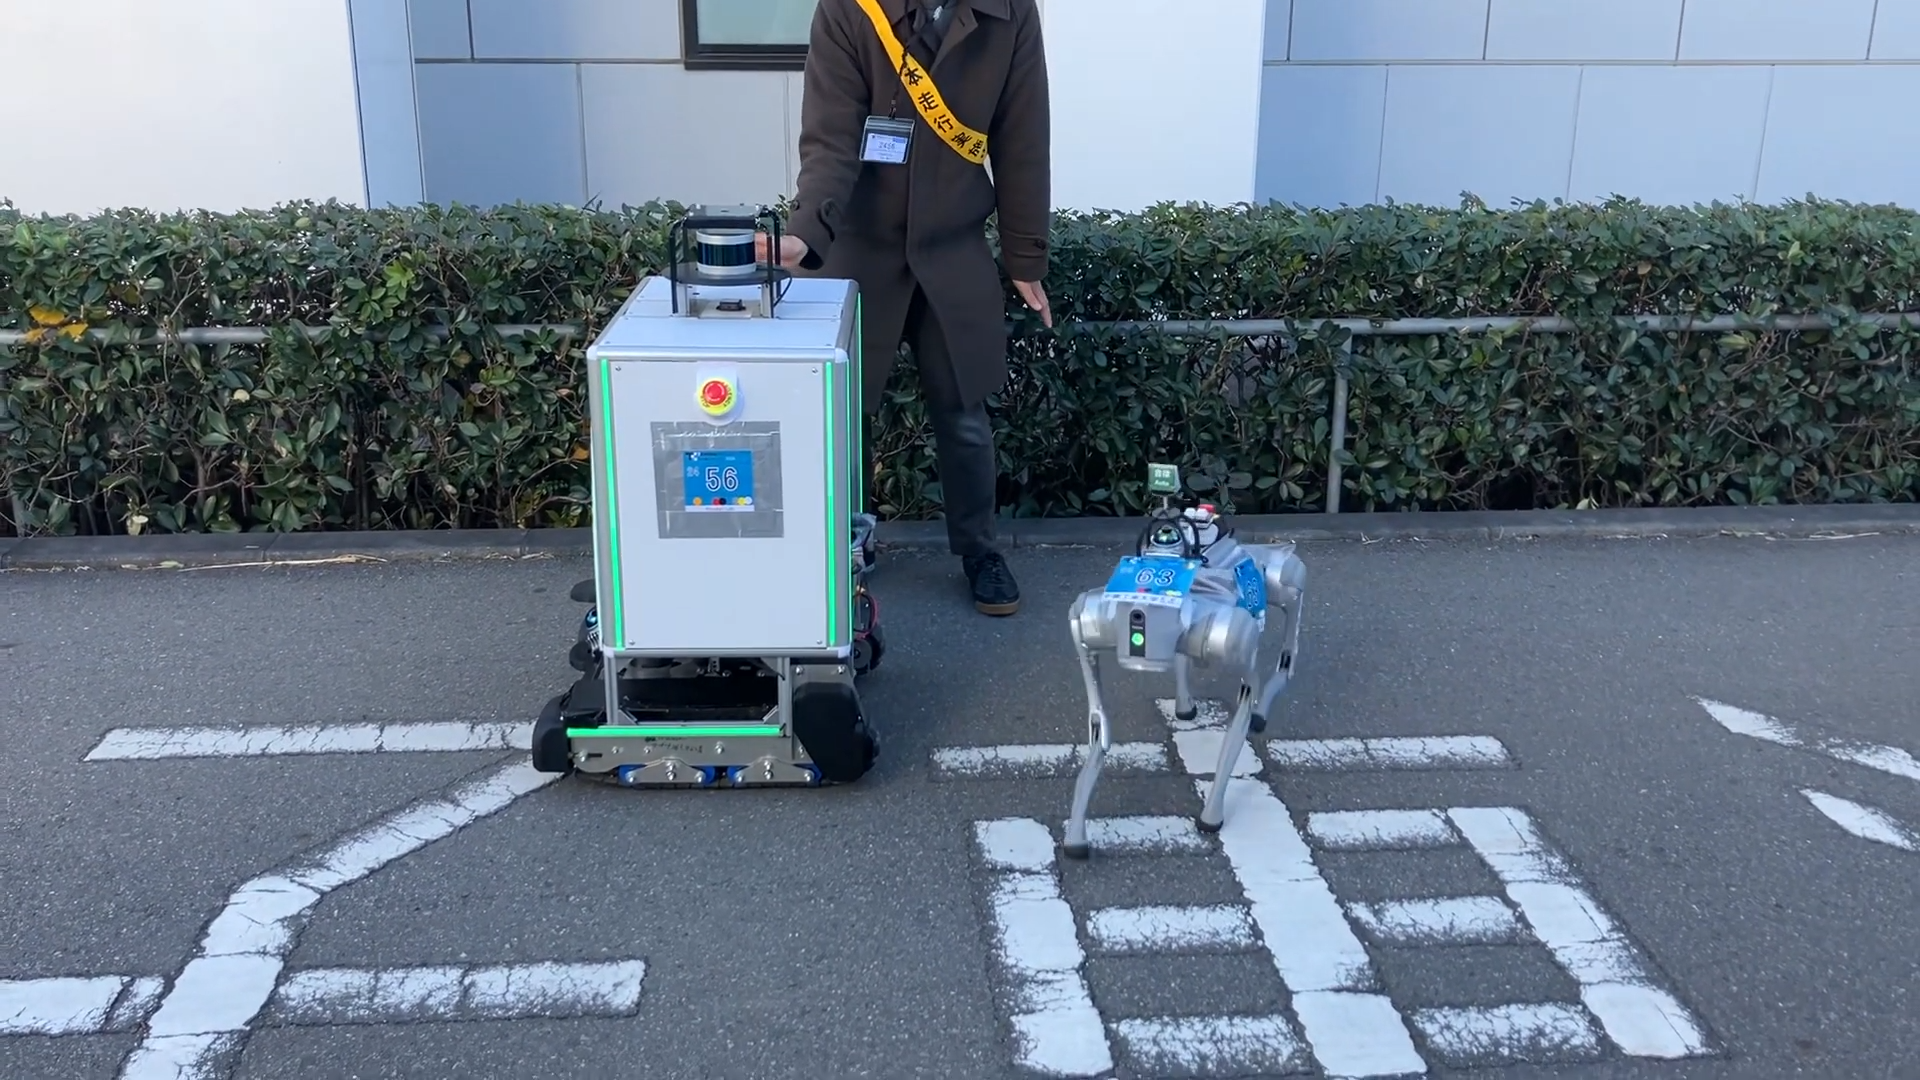
\includegraphics[width=\linewidth]{fig/honsoukou2.png}
        \caption{狭路が終わった段階で一時停止した時に、後続のロボットが追い越しを始める}
        \label{fig:honsoukou2}
        \end{minipage} \\

        \begin{minipage}[b]{0.45\hsize}
            \centering
            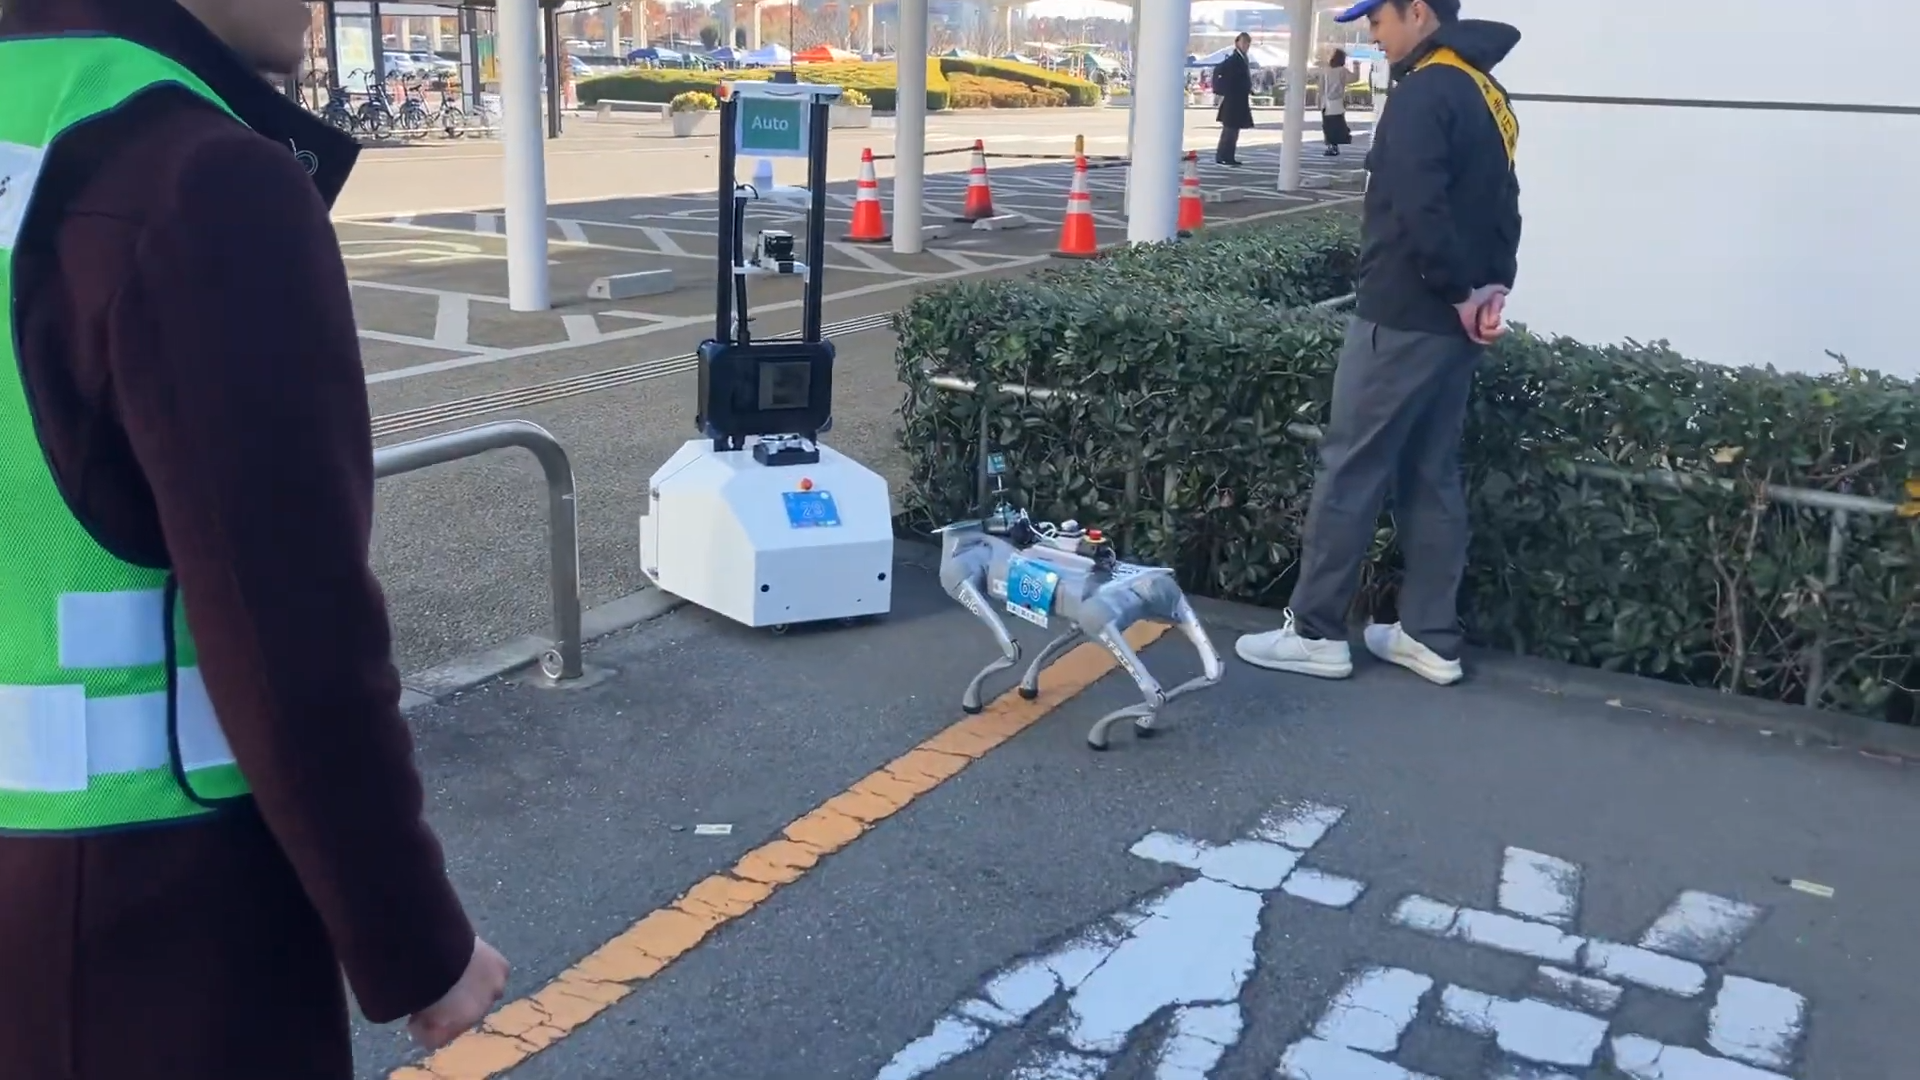
\includegraphics[width=\linewidth]{fig/honsoukou3.png}
            \caption{追い越したロボット同士で接触しそうになりしばらく停止}
            \label{fig:honsoukou3}
            \end{minipage} &
        %
            \begin{minipage}[b]{0.45\hsize}
            \centering
            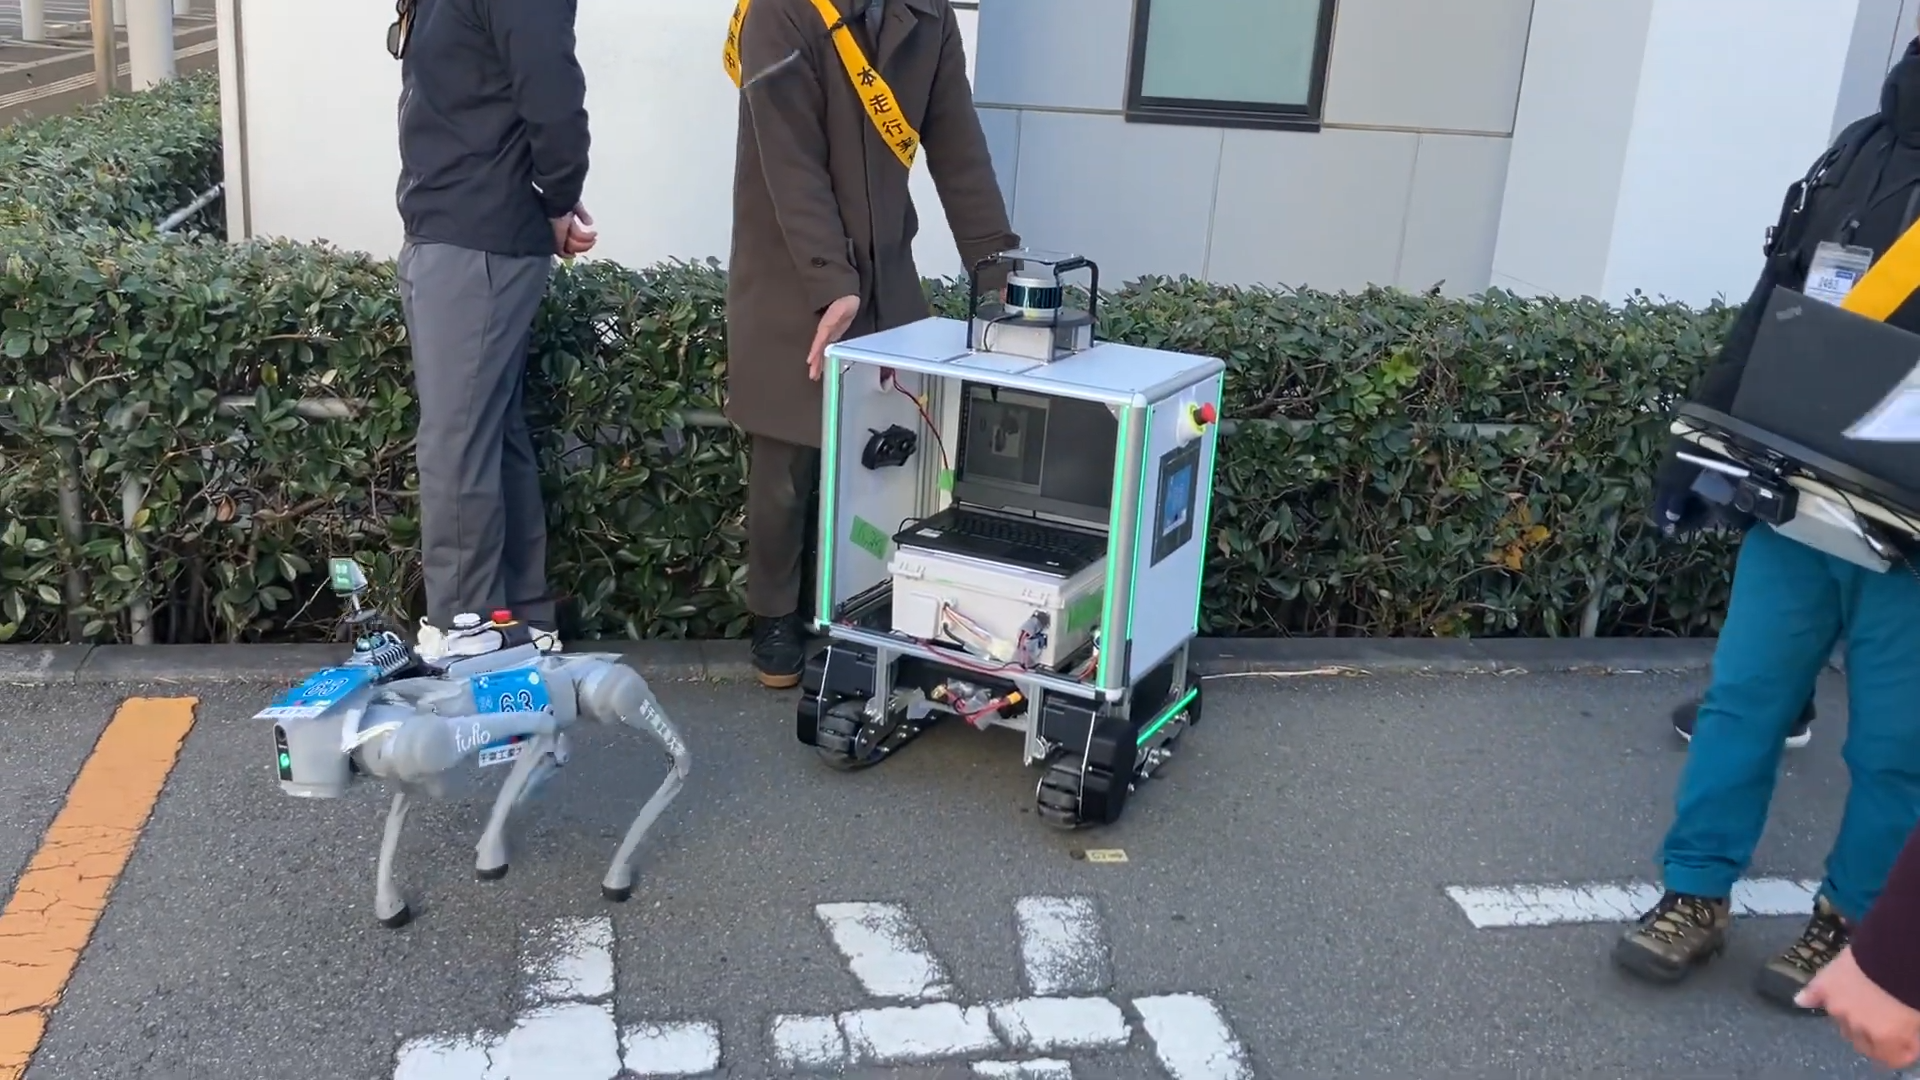
\includegraphics[width=\linewidth]{fig/honsoukou4.png}
            \caption{経路上にいるロボットを避けようとして壁に接近。復帰の経路作成できず断念}
            \label{fig:honsoukou4}
            \end{minipage}
    \end{tabular}
\end{figure*}
\section{本走行}
つくばチャレンジ2024の本走行では、市庁舎裏の細い通路でロボットを回避し、元の経路に再計画できずに180m地点でリタイアした。
それまでの走行は、自己位置を見失うこともなく、障害物を未検出になることなく動作した。

障害物からは距離を1m程度離れるように設定していたため、狭路で非常にゆっくり進んだ。
そのため、図\ref{fig:honsoukou1}のように後続のロボットが渋滞してしまった。

その後、図\ref{fig:honsoukou2}、\ref{fig:honsoukou3}のように、ロボットが追い越し、追い越され、経路上で詰まってしまった。
このロボットは設定したルートに忠実になぞる機能しか搭載していなかったゆえに、
迂回することができず、図\ref{fig:honsoukou4}のように障害物を回避したあと復帰できなくなった。

本年は確認走行区間内でリタイアしたが、
決められた座標の通りに走行する機能までは3DLiDARを使って実現することができた。
\section{結論}
つくばチャレンジ2024では、3DLiDARを利用したナビゲーションシステムを構築することができた。
3DLiDARのナビゲーションシステムは文献が少なく構築することに苦労したが、最低限の機能を揃えることはできた
つくばチャレンジの多くのロボットは3DLiDARを利用しているが、何から手をつければ良いかわからない人はいるはずである
このレポートでは、ハードウェアから自律ナビゲーションシステムの各機能のおおよその仕組みを述べた
来年初参加を考えている人の参考になれば幸いである
環境構築の方法や実際の詳細の使用方法などは引き続きブログで解説していく予定である。
次年度では、決められたルートを走行する上での意思決定機能を追加で実装する
完走するためには、不測の事態でも、認知判断行動することが必須である
完走にむけてナビゲーションシステムをブラッシュアップしていく予定である。

% 参考文献
\bibliographystyle{junsrt}
\bibliography{myrefs}

\end{document}
